%-------------------------------- Configurações --------------------------------

\documentclass[a4paper,         % Tamanho do papel: A4
	             abntfigtabnum,
	             noindentfirst,
	             normaltoc,
	             pnumplain,
	             notimes
	             % capchap,
]{abnt}

% Links border color
\newcommand{\bc}{NavyBlue}

\usepackage[utf8]{inputenc} % para pode escrever caracteres acentuados normalmente
\usepackage[brazil]{babel}
\usepackage{graphicx}
\usepackage[usenames,dvipsnames]{xcolor} % http://en.wikibooks.org/wiki/LaTeX/Colors
\usepackage[pdfborder={0 0 0},pdfborderstyle={/S/U/W 0.5},citebordercolor=\bc,filebordercolor=\bc,urlbordercolor=\bc,linkbordercolor=\bc]{hyperref} % http://www.tug.org/applications/hyperref/manual.html e http://migre.me/7FH3e
\usepackage[alf]{abntcite}
\usepackage{booktabs} % para utilização das linhas separadoras na tabela
\usepackage{textcomp}
\usepackage{minted} % foi adicionado o seguinte hack no minted: http://migre.me/7M8wI
\usepackage{nomencl} % para criar a lista de siglas

%--------------------------- Minted Highligthing -------------------------------

\renewcommand\listingscaption{Código}
\renewcommand{\nomname}{Lista de Siglas}

% http://github.com/hugomaiavieira/pygments-style-github
\usemintedstyle{github}

% O minted é tipo uma extensão do fancyvrb. Então, algumas modificações nele
% são feitas de acordo com o fancyvrb.
% Documentação do fancyvrb: http://linorg.usp.br/CTAN/macros/latex/contrib/fancyvrb/fancyvrb.pdf

% Ajustar o estilo do número, de acordo com o fancyvrb.
\renewcommand{\theFancyVerbLine}{\textcolor{Gray}{\scriptsize\arabic{FancyVerbLine}}}

% Ajusta estilo do caption. http://linorg.usp.br/CTAN/macros/latex/contrib/caption/caption-eng.pdf
\usepackage{caption}
\DeclareCaptionStyle{code_style}{justification=centering, skip=20pt}
\DeclareCaptionFont{all_label}{\footnotesize\bfseries}
\DeclareCaptionFont{all_text}{\footnotesize\upshape}
% captions dos códigos
\captionsetup[listing]{style=code_style,labelfont=all_label,textfont=all_text}
% todos os captions
\captionsetup{labelfont=all_label,textfont=all_text}

% Criando um novo comando para facilitar a adição de códigos
% http://tex.stackexchange.com/questions/42393/new-environment-with-minted
\makeatletter
\newenvironment{mycode}[3]
 {\VerbatimEnvironment
  \minted@resetoptions
  \setkeys{minted@opt}{linenos,fontfamily=courier, fontsize=\scriptsize, xleftmargin=21pt, frame=lines, framesep=5pt, framerule=1pt, numbersep=4pt}
  \renewcommand{\minted@proglang}[1]{#1}
    \captionof{listing}{#2\label{#3}} % http://migre.me/85CIT
      \begin{VerbatimOut}{\jobname.pyg}}
 {\end{VerbatimOut}
  \minted@pygmentize{\minted@proglang{}}
  \DeleteFile{\jobname.pyg}}
\makeatother

%------------------------- Numerar subsubsection -------------------------------

\makeatletter
\newcommand\sparagraph{\@startsection{section}{1}{\z@}%
                                    {3.25ex \@plus1ex \@minus.2ex}%
                                    {-1em}%
                                    {\normalfont\normalsize\bfseries}}
\newcommand\ssparagraph{\@startsection{subsection}{2}{\z@}%
                                    {3.25ex \@plus1ex \@minus.2ex}%
                                    {-1em}%
                                    {\normalfont\normalsize\bfseries}}
\newcommand\sssparagraph{\@startsection{subsubsection}{3}{\z@}%
                                    {3.25ex \@plus1ex \@minus.2ex}%
                                    {-1em}%
                                    {\normalfont\normalsize\bfseries}}
\setcounter{secnumdepth}{3}% Allow numbering up to \subsubsection or \sssparagraph
\makeatother

%----------------------- Quebra de linha após paragraph ------------------------

\makeatletter
\renewcommand\paragraph{\@startsection{paragraph}{4}{\z@}%
  {-3.25ex\@plus -1ex \@minus -.2ex}%
  {1.5ex \@plus .2ex}%
  {\normalfont\normalsize\bfseries}}
\makeatother

%--------------------------------- Informações ---------------------------------

\newcommand{\meutitulo}{Uso do Kanban-roots na contextualização de técnicas emergentes para teste de software}

% http://www.tug.org/applications/hyperref/manual.html
\hypersetup{
  pdftitle=\meutitulo,
  pdfauthor=Hugo Henriques Maia Vieira
}

\makenomenclature

\begin{document}

  \titulo{\meutitulo}
  \autor{Hugo Henriques Maia Vieira}
  \instituicao{Universidade Estadual do Norte Fluminense Darcy Ribeiro\par Laboratório de Ciências Matemáticas}
  \orientador[Orientadora:\par]{Profª. Drª. Annabell del Real Tamariz}
  \comentario{Monografia apresentada ao curso de graduação em Ciência da Computação da Universidade Estadual do Norte Fluminense Darcy Ribeiro como requisito para obtenção do título de Bacharel em Ciência da Computação.}
  \local{Campos dos Goytacazes - RJ}
  \data{2012}

  \capa
  \folhaderosto

  \begin{folhadeaprovacao}
  \thispagestyle{empty}
  \center
  \textbf{Hugo Henriques Maia Vieira}
  \vfill

  \center{\textbf{\Large{\textit{\meutitulo}}}}

  \hspace*{2cm}
  \begin{table}[h!]
    \raggedleft
    \begin{tabular}{p{7cm}}
    Monografia apresentada junto ao Curso de Ciência da Computação, da Universidade Estadual do Norte Fluminense Darcy Ribeiro – Campos / RJ, como requisito para obtenção do título de Bacharel em Ciência da Computação.
    Orientadora: Profª. Drª. Annabell del Real Tamariz.
    \end{tabular}
  \end{table}

  \hspace*{2cm}
  \raggedright Aprovado em 19/07/2012.

  \center
  \textbf{COMISSÃO EXAMINADORA}

  \setlength{\ABNTsignthickness}{0.4pt} \setlength{\ABNTsignskip}{1.7cm}

  \assinatura{Profª. Drª. Annabell del Real Tamariz \\ Orientadora - Universidade Estadual do Norte Fluminense Darcy Ribeiro}
  \assinatura{Prof. Dr. Rogério Atem de Carvalho \\ Instituto Federal Fluminense}
  \assinatura{Profª. Drª. Sahudy Montenegro González \\ Universidade Federal de São Carlos - Campos Sorocaba}
  \assinatura{Prof. Dr. Fermin Alfredo Tang Montané \\ Universidade Estadual do Norte Fluminense Darcy Ribeiro}
\end{folhadeaprovacao}
  \input{tex/epigrafe}
  \begin{center}
\textbf{AGRADECIMENTOS} \\ [2.5cm]
\end{center}

À meu pai Roosevelt, meu melhor amigo e grade companheiro, por estar sempre presente em todos os momentos felizes e tristes da minha vida e por ser a pessoa mais importante da formação do meu caráter, por eu me tornar quem sou.

À minha mãe e minhas irmãs, que mesmo distantes estão sempre por perto.

À minha namorada Alice, pelo amor, companheirismo e paciência.

Ao amigo e professor Rodrigo, por me mostrar o caminho da luz e por ser meu grande mestre e orientador.

À professora Sahudy, por ter sido parte fundamental da minha formação, acadêmica, profissional e pessoal.

À professora Annabell, por todo companheirismo e carinho, por mostrar que o trabalho duro é recompensador.

Ao professor Rivera por sua dedicação ao buscar sempre um curso melhor.

Ao professor Rogério, representando o NSI, por ter me aberto as portas para a área que adoro e escolhi seguir em minha vida profissional.

À todos meu amigos de curso, especialmente meus também companheiros de Algorich, Eduardo, Herond e Rafael por estarem presentes nos momentos mais dramáticos e nos mais engraçados.

À toda minha família, meus avós, meus primos e meus tios, por todo o suporte e felicidade que me proporcionam sempre.
  \begin{resumo}
Com a ascensão dos métodos ágeis de desenvolvimento nos últimos anos, diferentes técnicas de teste de software estão emergindo para dar suporte à principal característica de tais métodos: \textit{feedback} rápido. Baseado nisto, propomos neste trabalho contextualizar e discutir a utilização de técnicas emergentes de teste de software, enfocando as técnicas Desenvolvimento Guiado por Testes (do inglês, \textit{Test-Driven Development}), Desenvolvimento Guiado por Comportamento (do inglês, \textit{Behaviour-Driven Development}), Integração Contínua e Dublês de Teste, abordando-as em um estudo de caso, agregando conhecimentos, ainda dispersos e difusos, sobre as diferentes abordagens, possibilidades e pontos em aberto no emprego de tais técnicas, utilizando para isso o projeto kanban-roots.
\end{resumo}
  \begin{abstract}
With the rise of agile development methods in recent years, different software testing techniques are emerging to support the main feature of such methods: rapid feedback. Based on this, we propose in this work contextualise and discuss the use of emerging techniques for software testing, focusing on techniques Test-Driven Development, Behavior-Driven Development, Continuous Integration and Test Doubles, addressing them in a case study, adding knowledge, still scattered and diffuse, on different approaches, possibilities and open points use of such techniques, using for this project kanban-roots.
\end{abstract}

  \sumario
  \listoffigures
  \listoftables
  \printnomenclature

  \chapter{Introdução}

A tecnologia e os negócios mudam e evoluem de modo extremamente rápido hoje e o mercado demanda e espera software inovadores e de alta qualidade, que sejam adequados a suas necessidades e desenvolvidos o mais rápido possível \cite{TheBusinessOfInnovation}.

O desenvolvimento ágil de software, que neste ano de 2012 completa 11 anos, foi elaborado visando atender estas expectativas do mercado \cite{AgileManifesto}, focando o processo de desenvolvimento nas pessoas e abraçando as mudanças que naturalmente surgem durante o desenvolvimento do software.

Como a adoção do desenvolvimento ágil é crescente nos últimos anos \cite{ResumoChaosReport}, diversos métodos e técnicas vem sendo desenvolvidos, tendo como base os princípios e valores ágeis \cite{BDDRodrigo}, principalmente relacionadas ao teste de software. Contudo, estes métodos e técnicas continuam em evolução, tendo alguns de seus pontos ainda em aberto.

Este trabalho pretende contextualizar e discutir a utilização de técnicas emergentes de teste de software, aqui definidas como Desenvolvimento Guiado por Testes (do inglês, \textit{Test-Driven Development} - TDD)\nomenclature{TDD}{Test-Driven Development}, Desenvolvimento Guiado por Comportamento (do inglês, \textit{Behaviour-Driven Development - BDD})\nomenclature{BDD}{Behaviour-Driven Development}, Integração Contínua e Dublês de Teste. Para esta contextualização, será utilizado um sistema web desenvolvido pelo autor aplicando tais técnicas: o kanban-roots.

\section{Justificativas e objetivos}

São encontrados alguns poucos trabalhos relacionados ao tema abordado nesta monografia, como constata \citeonline{BDDSolis}. Sendo assim, o objetivo do presente trabalho é oferecer um estudo teórico-prático das técnicas emergentes na área de teste de software com metodologias ágeis de desenvolvimento, visando de agregar conhecimentos ora dispersos e difusos, sobre as diferentes abordagens, possibilidades e pontos em aberto no emprego de tais técnicas.

As técnicas que serão abordadas neste trabalho tiveram seu conceito definido no mercado e evoluem através da evolução das ferramentas que as implementam. Na figura \ref{img:fluxo_conceito_ferramenta} pode-se visualizar o fluxo de evolução onde primeiramente cria-se um conceito e, em seguida, uma ferramenta que o implemente. Com base na utilização e observação desta ferramenta, há uma percepção de novas necessidades, fazendo que os conceitos evoluam e novas ferramentas sejam criadas.

\begin{figure}[h]
  \center
  \caption{Fluxo de evolução dos conceitos e ferramentas}
  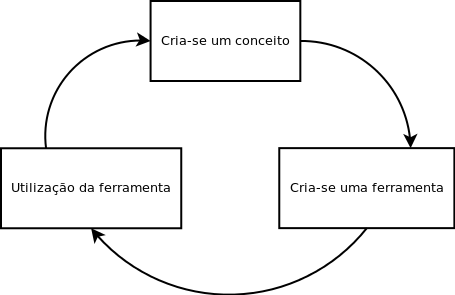
\includegraphics[scale=0.60]{images/fluxo-conceito-ferramenta}
  \label{img:fluxo_conceito_ferramenta}
\end{figure}

Desta forma, a evolução das ferramentas e a evolução conceitual estão intimamente ligadas. No texto original sobre BDD \cite{IntroducingBDD} já se encontra isto. A inspiração para a criação de BDD foi uma ferramenta chamada \textit{AgileDox}\footnote{Mais informações em \url{http://agiledox.sourceforge.net}}, que fez o autor da mesma antever as novas possibilidades que então cristalizou no conceito de BDD. Justamente por esta característica dinâmica de evolução, as informações e os diferentes conceitos sobre as técnicas estão dispersos, pois nunca foram sistematizados, ficando em uma espécie de ``inteligência coletiva"\ da comunidade de desenvolvimento ágil.

Além disso, como o presente trabalho está no contexto dos métodos ágeis, e nestes as partes conceitual e prática formam um todo inseparável, para toda técnica abordada serão exemplificados os conceitos usando o código de uma ferramenta web, denominada kanban-roots, desenvolvida pelo próprio autor do presente trabalho, utilizando práticas ágeis de desenvolvimento, especificamente Desenvolvimento guiado por Testes (TDD) e Desenvolvimento guiado por Comportamento (BDD).

\section{Metodologia}

Para atingirmos os objetivos propostos neste trabalho, será feita uma explanação sobre cada uma das técnicas emergentes estudadas, aqui definidas como:

\begin{itemize}
  \item Desenvolvimento guiado por testes (TDD, do inglês \textit{Test-Driven Development})
  \item Desenvolvimento guiado por comportamento (BDD, do inglês \textit{Behaviour-Driven Development}
  \item Integração contínua
  \item Dublês de teste
\end{itemize}

Serão comparadas as diferentes abordagens, possibilidades, pontos em aberto no emprego de cada técnica, observando a aplicabilidade de cada uma delas e a eficiência respectiva.

Como base para a discussão, será utilizado o kanban-roots\footnote{\url{http://github.com/hugomaiavieira/kanban-roots}}, que será apresentado na Seção \ref{sec:kanban_roots}. O kanban-roots é um projeto que foi desenvolvido pelo autor do presente trabalho utilizando todas as técnicas abordadas neste, possibilitando desta forma a obtenção de dados e experiências da utilização das técnicas em um projeto real.

Todos os trechos de código apresentados neste trabalho são trechos retirados do kanban-roots e a primeira linha de cada trecho sempre será um comentário informando o nome do arquivo original em que o referido trecho se encontra.

\section{Ferramentas utilizadas}

Para o desenvolvimento do kanban-roots foram utilizadas diversas ferramentas, sendo importante citar em que contexto e momento cada uma delas é utilizada.

Como base para o desenvolvimento, foi utilizado o \textit{framework web} Ruby On Rails\footnote{\url{http://rubyonrails.org}} que é escrito utilizando a linguagem de programação Ruby. Para os testes de unidade apresentados na Seção \ref{sub:tdd} foi utilizado o Test::Unit\footnote{\url{http://test-unit.rubyforge.org/}}. Já na Seção \ref{sub:bdd} é utilizado o Rspec\footnote{\url{http://rspec.info/}} para testes unitários, testes de aceitação e dublês de teste. Ainda na Seção \ref{sub:bdd} também foi utilizado o Cucumber\footnote{\url{http://cukes.info/}} para testes de aceitação. Além dessas ferramentas, também foi utilizado o FactoryGirl\footnote{\url{https://github.com/thoughtbot/factory_girl}} para \textit{fixtures replacement} em todos os momentos em que se fez necessário. Foram ainda utilizados os banco de dados SQLite\footnote{\url{http://www.sqlite.org/}}, em ambiente de desenvolvimento, e o MySQL\footnote{\url{http://www.mysql.com}}, em ambiente de produção.

\section{Organização}
\label{sec:organizacao}

No Capítulo 2 será fundamentado os diferentes tipos de teste de software bem como as técnicas emergentes abordadas no presente trabalho. No Capítulo 3 serão contextualizadas as técnicas emergentes de teste de software, discutindo suas abordagens e pontos em aberto. No Capítulo 4 são apresentadas as conclusões obtidas e os trabalhos futuros.
  \chapter{Fundamentação teórica}

\section{Desenvolvimento de software}
\label{sec:desenvolvimento_de_software}

O desenvolvimento de software é o ato de elaborar e implementar um sistema computacional que transforme as necessidades de um utilizador ou de um mercado em um produto de software.

O desenvolvimento de software é essencialmente uma atividade intelectual e criativa, exigindo a manipulação de uma gama muito grande de conhecimentos e informações. Além disso, os desenvolvedores de um software se preocuparem com o conteúdo e estrutura, além de deverem se preocupar também com o comportamento fazendo com o que o desenvolvimento de software seja uma atividade complexa, devendo ser realizada por especialistas munidos de técnicas que os auxiliem da melhor maneira possível.


\subsection{Agilismo}
\label{sub:agilismo}

Em 2001 um grupo de dezessete especialistas, reconhecidos pela comunidade como grandes nomes do desenvolvimento software, se reuniram para discutir sobre um crescente conjunto de métodos que vinham surgindo e decidiram usar o termo Agilismo para descrever essa nova geração de métodos \cite{AgileStory}. Na mesma reunião, eles também escreveram o Manifesto Ágil \cite{AgileManifesto}, delineando um conjunto de valores e princípios que, em resumo, trilham um caminho para a eliminação de documentação e processos desnecessários, buscando a simplicidade, com foco na geração de valor e proximidade com o cliente, além de possibilitar respostas rápidas e eficazes às mudanças. Desde então, os métodos ágeis vêm ganhando projeção e importância no cenário da produção de software.

Pode-se dizer então, que o Desenvolvimento Ágil, ou Agilismo, é um rótulo genérico para os métodos de desenvolvimento de software baseados no Manifesto Ágil.

É importante citar que o desenvolvimento ágil sofreu grande influência de um conceito conhecido como \textit{Lean Thinking} (``pensamento enxuto"\ em português), uma linha de pensamento em gestão baseada nos princípios de \textit{Lean Manufacturing}\footnote{Os princípios de \textit{Lean Manufacturing} são originários do sistema Toyota de produção, que propôs um modo inteiramente novo de pensar a respeito de fabricação e logística de automóveis.} que se caracteriza por produção em pequenos lotes, eliminação de desperdícios, obsessão com qualidade, equipes multifuncionais praticando aprendizado contínuo, melhoria contínua de processo, sistema puxado de produção e a qualidade sendo responsabilidade dos trabalhadores como um todo \cite{BDDRodrigo}.

Uma das premissas do agilismo é que os custos de alterações sejam praticamente linear ao longo do tempo, independente do ponto em que esteja, fazendo com que a curva de custo de alterações seja semelhante à apresentada na Figura \ref{img:custo-agile}.

\begin{figure}[h]
  \center
  \caption{O custo das modificações no modelo ágil - Fonte: \cite{XPKent}}
  \includegraphics[scale=0.45]{images/custo-agile}
  \label{img:custo-agile}
\end{figure}

Isto é conseguido porque nos métodos ágeis não é feito um planejamento inicial muito abrangente. Ao invés disso, o desenvolvimento é dividido em iterações curtas (de uma a quatro semanas), onde ao início de cada uma delas é feito um novo planejamento, corrigindo o curso do projeto com base no \textit{feedback} obtido nas iterações anteriores. Para isso, a proximidade e interação do cliente com o projeto deve ser constante. Desta forma, o desenvolvimento é baseado em \textit{feedback} concreto e não em especulações sobre o futuro, fazendo com que o aprendizado permanente leve a melhorias e torne o produto final mais adequado para o seu público, além de o tornar mais simples e sem elementos extras que poderiam ser utilizados no futuro. Além disso, os testes automatizados são fundamentais para que as modificações realizadas não alterem o comportamento atual do sistema  \cite{XPKent}, dando segurança para que estas sejam feitas, além de permitir que o código melhore continuamente.

Ao utilizar métodos ágeis como \textit{eXtreme Programming} (XP) \nomenclature{XP}{eXtreme Programming} e Scrum, todas as funcionalidades do sistema são levantadas através de histórias, que são escritas pelo próprio cliente em pequenos cartões. A equipe de desenvolvimento utiliza os cartões para saber quais funcionalidades são desejadas pelo cliente. Contudo, os cartões podem acabar representando histórias que consomem muito esforço para serem implementadas. Nesse caso, a equipe divide os cartões em tarefas, que são registradas em novos cartões para serem distribuídas facilmente entre os desenvolvedores. Na Figura \ref{img:projeto_agile} é mostrada divisão de um projeto nos métodos ágeis.

\begin{figure}[h]
  \center
  \caption{Divisão de um projeto nos métodos ágeis}
  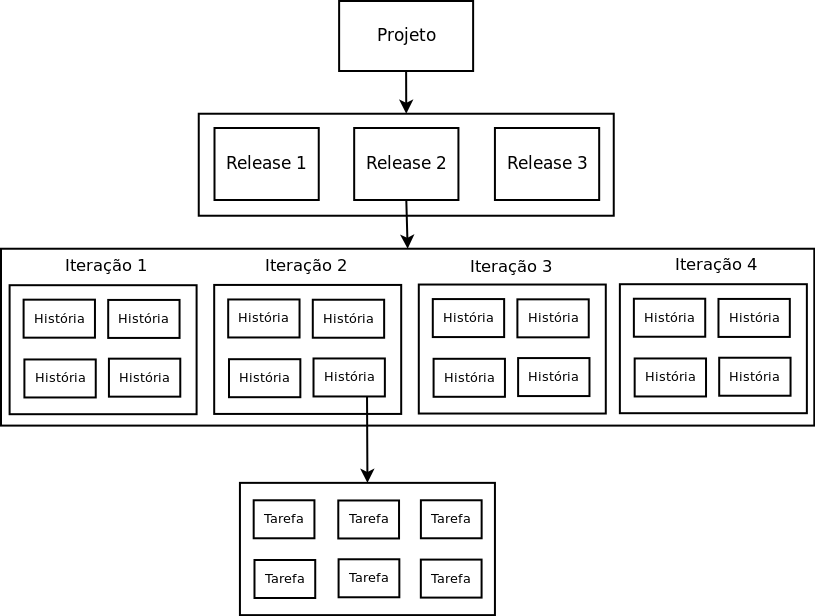
\includegraphics[scale=0.45]{images/projeto}
  \label{img:projeto_agile}
\end{figure}

No início do projeto o cliente e a equipe de desenvolvimento dividem o projeto em \textit{releases}, que são entregas de software que implementem um conjunto de funcionalidades que possui um valor bem definido para o cliente. Essas entregas são feitas de forma incremental, e em um espaço de tempo não muito longo (geralmente dois meses), para que o cliente possa começar a utilizar e obter os benefícios que elas oferecem, além de dar o \textit{feedback} necessário para que sejam feitas melhorias. Depois de definida a primeira \textit{release}, o cliente escreve as histórias que serão implementas nesta. As histórias das \textit{releases} posteriores podem ser deixadas para o futuro, pois durante o desenvolvimento de cada \textit{release} o cliente irá utilizar o software diversas vezes, o que irá influenciar as histórias das próximas \textit{release}. Durante a \textit{release} o cliente pode alterar as histórias se considerar necessário, podendo assim incorporar o aprendizado adquirido com o uso do sistema.

Uma \textit{release}, mesmo que seja pequena, representa um tempo ainda grande, pois não se deve esperar tanto tempo para ter o \textit{feedback} da utilização do software pelo cliente. Assim, ela é dividida em um conjunto de iterações, que são basicamente um pequeno espaço de tempo (geralmente duas semanas) dedicado para a implementação de um conjunto de histórias. A diferença entre uma \textit{release} e uma iteração é que na iteração o cliente não pode alterar as histórias definidas, pois a mudanças muito frequentes ao longo do trabalho da equipe de desenvolvimento prejudicam o ritmo de programação, pois confundem os desenvolvedores. No início de cara iteração é feita uma reunião para o planejamento da mesma, de modo que cliente e equipe de desenvolvimento definam as histórias que serão implementadas na iteração. Ao final de cada iteração e cada \textit{release}, o cliente tem novas histórias implementadas, ou seja, software funcionando. Dessa forma, ele poderá utilizar o sistema com as novas funcionalidades, tornando o \textit{feedback} ainda mais efetivo.

Mas para que isso seja possível, os métodos ágeis contam com um conjunto de técnicas para dar suporte a seu caráter iterativo e incremental, sendo algumas destas técnicas abordadas mais adiante neste trabalho.


\section{Teste de software}
\label{sec:teste_de_software}

A maneira como o teste de software é aplicado varia de acordo com a metodologia utilizada no desenvolvimento. Tradicionalmente o teste de software é feito somente após o desenvolvimento ter sido concluído \cite{TesteSoftware, Pressman}. Já nos métodos ágeis um sentido oposto é seguido \cite{ArtOfAgileDevelopment}, sendo utilizadas técnicas como \textit{Test-Driven Development} (abordada na Seção \ref{sub:tdd}) e \textit{Behaviour-Driven Development} (abordada na Seção \ref{sub:bdd}).

O uso de estratégias nas quais a escrita dos testes automatizados é feita antes do código de implementação das funcionalidades, como TDD e BDD, não exclui o emprego de técnicas de teste de software tradicionais como classes de equivalência, análise do valor limite, análise da complexidade ciclomática e outras.

Os próximos tópicos definirão os tipos de teste utilizados no contexto do presente trabalho.


\subsection{Testes de unidade}
\label{sub:testes_de_unidade}

Testes de unidade são testes nos quais unidades individuais do sistema são testadas para determinar se estão aptas para uso. Uma unidade é a menor parte testável de uma aplicação. Em programação procedural uma unidade pode ser uma função. Já em programação orientada a objetos, uma unidade pode ser um método ou uma responsabilidade da classe. \citeonline{TesteSoftware} afirmam que neste contexto, espera-se que sejam identificados erros relacionados a algoritmos incorretos ou mal implementados, estruturas de dados incorretas, ou simplesmente erros de programação.

Para exemplificar, no Código \ref{code:unit_test_spec} é apresentado o teste de unidade para o método \texttt{Category\#name\_as\_css\_class}, cuja implementação é mostrada no Código \ref{code:unit_test}. Este método transforma o nome da Categoria em um nome de classe CSS\footnote{\textit{Cascading Style Sheets}. Mais em \url{http://pt.wikipedia.org/wiki/Cascading_Style_Sheets}}\nomenclature{CSS}{Cascading Style Sheets}, deixando todos seus caracteres em minúsculo e substituindo os caracteres / (barra),  (espaço) e - (traço) por \_ (sublinhado).

\begin{mycode}{rspec}%
{Teste de unidade automatizado para o método \texttt{Category\#name\_as\_css\_class} }{code:unit_test_spec}
# spec/models/category_spec.rb
describe Category do
  it "should return its name as a css class" do
    category = Factory.build :category, :name => "Feature"
    category.name_as_css_class.should == "feature"

    category.name = "New Feature"
    category.name_as_css_class.should == "new_feature"

    category.name = "Other-New Feature"
    category.name_as_css_class.should == "other_new_feature"

    category.name = "Study/Research"
    category.name_as_css_class.should == "study_research"
  end
end
\end{mycode}

\begin{mycode}{rspec}%
{Implementação do método \texttt{Category\#name\_as\_css\_class} }{code:unit_test}
# app/models/category.rb
class Category < ActiveRecord::Base
  def name_as_css_class
    self.name.downcase.gsub(/\/| |-/, "_")
  end
end
\end{mycode}


\subsection{Testes de integração}
\label{sub:testes_de_integracao}

No contexto do presente trabalho, os testes de integração testam as integrações do código com o mundo exterior. Eles podem ser testes que se comuniquem através da rede, tenham contato com o sistema de arquivos ou deixem os limites de seu próprio processo \cite{ArtOfAgileDevelopment}.

Para exemplificar, será utilizada uma extensão criada para fazer o destaque da sintaxe de código na descrição das Tarefas e no conteúdo do Comentários no kanban-roots, como apresentado na Figura \ref{img:highlighting}. Para isso, é utilizado um \textit{framework} em Python chamado Pygments\footnote{ Mais em \url{http://pygments.org/}}.

\begin{figure}[h]
  \center
  \caption{Comentário com destaque da sintaxe de código no kanban-roots}
  \includegraphics[scale=0.5]{images/highlighting}
  \label{img:highlighting}
\end{figure}

O Pygments deve ser instalado na máquina onde o kanban-roots está sendo executado. No entanto, o kanban-roots foi projetado rodar em um servidor próprio ou em um VPS\footnote{ \textit{Virtual Private Server}. É um servidor em ambiente compartilhado que possui acesso \textit{root} e processos independentes para cada conta VPS criada.}, mas também no Heroku\footnote{ É um PaaS (\textit{platafom as a service}) que tem uma cota de utilização gratuita. No Heroku não é possível instalar dependências no sistema. Mais em \url{http://heroku.com}}. Sendo assim, foi utilizado um serviço gratuito e não oficial criado por Trevor Turk e hospedado no Google App Engine que permite a utilização da API \nomenclature{API}{Application programming interface} do Pygments através de um POST para o serviço. Dessa forma, deve-se testar a integração com o serviço e também a integração com o Pygments instalado localmente.

No Código \ref{code:integration_spec} é apresentado o teste de integração para o \textit{highlighting} de código englobando os dois casos citados anteriormente e no Código \ref{code:integration} é apresentada a implementação para esta fucnionalidade.

É importante perceber que, para isolar o teste, foi utilizado um dublê de teste (neste caso um \textit{stub}) para simular a resposta do método \texttt{can\_pygmentize?} que faz uma verificação no sistema operacional para identificar se o Pygments está instalado ou não. Dublês de teste serão abordados mais detalhadamente na Seção \ref{sub:dubles_de_teste}.

\begin{mycode}{rspec}%
{Teste de integração automatizado para o \textit{highlighting} de código}{code:integration_spec}
# spec/lib/albino_render_spec.rb
describe HTMLwithAlbino do
  before(:all) do
    @render = HTMLwithAlbino.new
    @code_text = 'puts "hello!"'
    @highlighted_code =
      "<div class=\"highlight\"><pre>" +
        "<span class=\"nb\">puts</span> <span class=\"s2\">&quot;hello!&quot;</span>\n" +
      "</pre>\n</div>\n"
  end

  it "should get the highlighted block code from pygments.appspot.com" do
    @render.stub(:can_pygmentize?).and_return(false)
    @render.block_code(@code_text, "ruby").should == @highlighted_code
  end

  it "should get the highlighted block code from local pygments" do
    @render.stub(:can_pygmentize?).and_return(true)
    @render.block_code(@code_text, "ruby").should == @highlighted_code
  end
end
\end{mycode}

\begin{mycode}{ruby}%
{Implementação do \textit{highlighting} de código}{code:integration}
# lib/albino_render.rb
class HTMLwithAlbino < Redcarpet::Render::HTML
  def block_code(code, lang)
    if can_pygmentize?
      Albino.colorize(code, lang)
    else
      # This is a hack for pygments work on Heroku
      require "net/http"
      Net::HTTP.post_form(URI.parse("http://pygments.appspot.com/"),
                          {"code"=>code, "lang"=>lang}).body
    end
  end

  private
  def can_pygmentize?
    system "pygmentize -V"
  end
end
\end{mycode}


\subsection{Testes de aceitação}
\label{ssub:testes_de_aceitacao}

Testes de aceitação são especificações para o comportamento das funcionalidades de um sistema. Eles mostram se o sistema se comporta corretamente pela perspectiva de um usuário, sem nos dizer nada sobre como o sistema implementa esse comportamento \cite{TestDrivenKoskela}. Além disso, é verificada a integração entre as diversas unidades que interagem para prover esta funcionalidade.

Relacionando com os métodos tradicionais, os testes de aceitação implementam os casos de uso levantados na análise orientada a objetos.

No Código \ref{code:acceptance} são apresentados exemplos de teste de aceitação, utilizando BDD com a escrita em texto plano. O primeiro cenário testa a funcionalidade de clicar e arrartar as tarefas de uma posição para outra no kanban. Já o segundo cenário testa a funcionalidade de limpar a divisão \textit{Done} do kanban, ou seja, retirar do quadro todas as tarefas concluídas.

BDD e testes de aceitação serão vistos com mais detalhes na Seção \ref{sub:bdd}.

\begin{mycode}{cucumber}%
{Teste de aceitação para o registro de um contribuidor}{code:acceptance}
# features/board.feature
Feature: Use the board
  As a user
  I want use the board
  In order see, move and manipulate the taks of my project

  @javascript
  Scenario: Drag and drop a task to another board position
    Given I am an authenticated contributor
    And I have a project
    And the following tasks:
      | title  | position |
      | task 1 | Doing    |
      | task 2 | Done     |
    And I am on the projects board page
    When I drag "task 1" task to "Done" position
    Then I should see "task 1" task at "Done" position

  Scenario: Clean up Done tasks
    Given I am an authenticated contributor
    And I have a project
    And the following tasks:
      | title  | position |
      | task 1 | Doing    |
      | task 2 | Done     |
      | task 3 | Done     |
      | task 4 | Done     |
    When I am on the projects board page
    And I follow "Clean up Done"
    Then I should see "Done division was cleaned up."
    And the Done division should be cleaned
\end{mycode}


\section{Técnicas emergentes de teste de software}
\label{sec:tecnicas_emergentes_de_teste_de_software}

Nesta seção serão apresentadas, conceitualmente, as técnicas emergentes de teste de software, sendo elas o Desenvolvimento Guiado por Testes (do inglês, \textit{Test-Driven Development} - TDD), Desenvolvimento Guiado por Comportamento (do inglês, \textit{Behaviour-Driven Development - BDD}), Integração Contínua e Dublês de Teste.

\subsection{Test-Driven Development (TDD)}
\label{sub:tdd}

O \textit{Test-Driven Development} (Desenvolvimento guiado por testes) é uma técnica onde o desenvolvimento do software é guiado por \textbf{testes automatizados}, que são escritos antes de qualquer linha de código relativo a funcionalidades. Primeiro escreve-se um teste, depois escreve-se o código para passar neste teste. Em seguida, o código é refatorado para encontrar um design melhor, contando sempre com os testes existentes para que não sejam introduzidas falhas em outras partes do sistema.

Esta abordagem encoraja bom design \cite{GrowingOOByTests}, produz código testável e mantém longe a sobre-engenharia por conta de falsas suposições, pois, nos testes, é especificado o que é desejado e escreve-se o código para fazer apenas aquilo que realmente é necessário. \cite{TestDrivenKoskela, TDDbyExample, EmpiricalTDD}

\citeonline{EmergentDesign} relaciona o entendimento do problema e o fluxo natural do TDD:

\begin{citacao}
Tentar escrever um teste é uma boa maneira de testar a si mesmo sobre seu conhecimento sobre como a classe deverá funcionar antes de você escrevê-la. Esta é uma boa sequência: tenha certeza de que você entende o que você irá tentar fazer antes de você realmente tentar fazer. De fato, colocando dessa maneira, parece muito mais natural considerar os testes como Primeira Tarefa e criar o código como Segunda Tarefa. (tradução do autor)
\end{citacao}

O TDD vem sendo utilizado esporadicamente há anos, contudo, não existia um nome para identificar essa forma de desenvolver software, que no fim dos anos noventa, ganhou além do nome, uma definição. Atualmente, TDD começa a ganhar força e ser utilizada em times de grandes empresas como Google, Yahoo, Microsoft e IBM \cite{EmpiricalTDD}. O Anexo \ref{cha:a_efetividade_do_tdd} apresenta uma análise de diversos estudos sobre a efetividade de TDD na indústria e na academia.

\subsubsection{Ciclo TDD}
\label{ssub:ciclo_tdd}

Com base no trabalho de \citeonline{TDDbyExample}, o ciclo de desenvolvimento TDD é composto pelas seguintes etapas:

\begin{enumerate}
\item \textbf{Adicionar um teste}

Cada ciclo se inicia com a criação de um teste de unidade. Este teste inevitavelmente irá falhar, pois é escrito antes do código ser implementado de fato. Para escrever um teste, o desenvolvedor precisa entender claramente as especificações e requisitos da unidade. Isso faz com que o desenvolvedor tenha como foco os requisitos antes do código, o direcionando a escrever código apenas para o que é realmente necessário.

Além disso, segundo \citeonline{XPTeles}, ao se pensar e escrever o teste, está sendo feita também a análise e \textit{design} das classes do sistema.

\item \textbf{Executar todos os testes e ver se algum falha}

Todos os testes devem ser executados e o novo teste deve falhar pela razão esperada: a funcionalidade não foi desenvolvida. Isto aumenta a confiança que se está testando a coisa certa.

\item \textbf{Escrever código}

O próximo passo é escrever código \textbf{somente para que o teste passe}. O código poderá não ser perfeito, pois posteriormente ele será melhorado. O importante é que o código faça o mínimo para passar no teste. Segundo \citeonline{BDDRodrigo}:

\begin{citacao}
Enquanto código útil é um patrimônio que gera valor, qualquer código criado inutilmente é tempo desperdiçado e, no fim das contas, um fardo, que sem gerar valor algum, aumentará a complexidade geral do software.
\end{citacao}

\item \textbf{Executar os testes e ter sucesso}

Ao Executar os testes e todos eles passarem, o código possuirá todos os requisitos testados e o programador pode ficar confiante para melhorá-lo.

\item \textbf{Refatorar}

Esta é uma etapa muito importante, onde o código escrito anteriormente é melhorado. Segundo \citeonline{FowlerRefatoracao}, refatorar é reestruturar o software aplicando uma série de alterações em sua estrutura interna para torná-lo mais fácil de ser entendido e menos custoso de ser modificado, sem alterar seu comportamento observável.

Refatorar melhora o projeto do software, o torna mais fácil de entender e modificar, ajuda a encontrar falhas e ajuda o desenvolvedor a programar mais rapidamente.

Como na refatoração o comportamento do código não deve ser alterado, após refatorar e executar novamente os testes, todos eles devem passar.

\end{enumerate}

A figura \ref{img:ciclo-tdd} resume o ciclo TDD, onde as etapas 1 e 2 são representadas pelo item \textbf{teste}, as etapas 3 e 4 pelo item \textbf{codifique} e a etapa 5 pelo item \textbf{refatore}.

\begin{figure}[h]
  \center
  \caption{O ciclo TDD}
  \includegraphics[scale=0.45]{images/ciclo-tdd}
  \label{img:ciclo-tdd}
\end{figure}


\subsubsection{Design emergente}
\label{ssub:design_emergente}

\textbf{TODO: juntar isso com o mesmo tópico em contextualização?}

No contexto em que TDD costuma ser aplicado $-$ em processos ágeis, com um ciclo de vida iterativo-incremental $-$ não é realizado um amplo \textit{design} prévio. Sendo assim, o \textit{design} evolui incrementalmente, ou seja, o \textit{design} emerge de acordo com a necessidade. Sabendo disso, uma característica extremamente importante do TDD é a facilitação ao \textit{design} emergente, que muitos consideram ser sua a principal característica \cite{EmergentDesign}.

TDD é considerada uma técnica essencial para o \textit{design} emergente porque
quando se está escrevendo um teste anteriormente ao código, o programador contempla e decide não apenas a interface do software (i.e. nomes de classes/métodos, parâmetros, tipos de retorno, lançamento de exceções), mas também o comportamento do software (i.e. resultados esperados para determinadas entradas) \cite{JanzenTDD}.

Além disso, \citeonline{EmergentDesign} constata que o ponto de vista do teste pode passar informações sobre o design, porque o teste de uma classe funciona como o primeiro cliente da classe. Com isso, a interface que o teste sugere é uma interface dirigida ao cliente, sendo assim, geralmente é mais estável.

\citeonline{DammTDD} também afirmam que o TDD faz com que as pessoas pensem mais no design em vez de codificar precipitadamente sem saber o que implementar ainda e \citeonline{XPTeles} ressalta a importância da refatoração para a evolução incremental do design:

\begin{citacao}
Ao longo das iterações, o design precisa evoluir, mas deve manter-se simples e claro para que a equipe possa fazer alterações no software a qualquer momento, com facilidade. Por esta razão o \textit{refactoring} tem um papel fundamental no design.
\end{citacao}


\subsection{Behaviour-Driven Development (BDD)}
\label{sub:bdd}

Criado em 2006 \cite{IntroducingBDD}, \textit{Behaviour-Driven Development} (Desenvolvimento guiado por comportamento) é uma técnica de desenvolvimento de software cuja amplitude se estende às atividades de design, documentação, validação e verificação, tratando-as de modo unificado \cite{BDDRodrigo}.

O Principal objetivo do BDD é ter especificações (também consideradas documentações) executáveis do sistema. Tudo que foi dito anteriormente sobre TDD vale também para BDD, mas em BDD os testes são escritos de forma mais clara e são mais facilmente lidos, pois BDD provê uma \textit{ubiquitous language} baseada no domínio do problema. Com isso, o vocabulário do problema (negócios) permeia diretamente para o código \cite{IntroducingBDD}.

\subsubsection{Ubiquitous Language}
\label{ssub:ubiquitous_language}

Uma \textit{ubiquitous language} é uma linguagem baseada no domínio do negócio, permitindo que clientes e desenvolvedores falem a mesma língua sem ambiguidade. Segundo \citeonline{BDDSolis}, o conceito de \textit{ubiquitous language} é o núcleo do BDD.


\citeonline{DDD} diz que uma \textit{ubiquitous language} é uma linguagem comum a todo o projeto, cobrindo toda acadeia de comunicação, desde conversas entre o cliente e o analista de negócios até conversas internas da equipe de desenvolvimento, chegando aos termos utilizados no código e mesmo nas estruturas de banco de dados.

Dessa forma, uma \textit{ubiquitous language} estreita a colaboração entre clientes e desenvolvedores, ao facilitar a comunicação e o \textit{feedback} \cite{DDD}.

\subsubsection{O ciclo BDD}
\label{ssub:o_ciclo_bdd}

O Ciclo BDD (também chamado de ciclo \textit{outside-in}\footnote{O ciclo recebe este nome devido à sequência que deve ser percorrida, que se inicia dos requisitos e da visão do cliente (\textit{outside}) até as entranhas dos artefatos de software (\textit{in}) \cite{BDDRodrigo}.}), apresentado na Figura \ref{img:ciclo-bdd}, tem dois níveis: unidade e aceitação. O nível aceitação é o nível mais alto, onde são escritos os testes de aceitação. Já o nível unidade é o mesmíssimo \hyperref[ssub:ciclo_tdd]{ciclo TDD} visto anteriormente. Este ciclo pode ser explicado na seguinte série de passos:

\begin{enumerate}
\item \textbf{Adicionar um teste de aceitação com foco em um cenário}

Cada ciclo se inicia com a criação de um teste de aceitação, tendo como foco um cenário que descreve um determinado comportamento de uma funcionalidade do sistema. Para fazer um paralelo com os métodos tradicionais de desenvolvimento de software, pode-se ver os cenários como casos de uso.

\citeonline{BDDRodrigo} define como que, em BDD, o foco do desenvolvedor deve estar em um único cenário por vez, e os benefícios dessa abordagem:

\begin{citacao}
Na terminologia de BDD, um cenário é um exemplo de utilização de uma dada funcionalidade. Uma funcionalidade é algo que o software deve oferecer e que possui um valor bem definido para o cliente. Em BDD, o foco dos desenvolvedores deve estar sempre direcionado à um único cenário de uma única funcionalidade por vez. Isto elimina dispersões e mantém o desenvolvedor concentrado na tarefa a ser realizada. Um desenvolvedor utilizando BDD deve encarar um novo cenário como se todos os requisitos do software fossem apenas os cenários já implementados e o atual, ou seja, não se preocupará, no momento, com as próximas funcionalidades ou cenários. Isto é importante para evitar generalizações baseadas em especulações a respeito do que o software possa eventualmente necessitar no futuro, o que aumenta a complexidade do \textit{design} sem qualquer garantia de que será realmente útil.
\end{citacao}

\item \textbf{Executar todos os testes e ver se algum falha}

Assim como no \hyperref[ssub:ciclo_tdd]{ciclo TDD}, todos os testes devem ser executados e o novo teste deve falhar pela razão pois a funcionalidade ainda não foi desenvolvida.

\item \textbf{Descer de nível}

Neste momento, deve-se descer de nível, saindo do nível de aceitação e indo para nível de unidade.

\item \textbf{Entra no ciclo TDD}

No nível de unidade, entra-se no \hyperref[ssub:ciclo_tdd]{ciclo TDD} até que todos os testes de unidade estejam passando.

\item \textbf{Retornar para o nível de aceitação}

Com todos os testes de unidade passando, retorna-se para o nível de aceitação e faz-se todos os testes deste nível passarem.

\item \textbf{Refatorar}

Neste passo, é feita a refatoração do código, da mesma maneira como é feita no \hyperref[ssub:ciclo_tdd]{ciclo TDD}.

\end{enumerate}

\begin{figure}[h]
  \center
  \caption{O ciclo BDD}
  \includegraphics[scale=0.45]{images/ciclo-bdd}
  \label{img:ciclo-bdd}
\end{figure}

\subsection{Integração contínua}
\label{sub:integracao_continua}

Em uma equipe com vários desenvolvedores, todos trabalhando na elaboração de um mesmo sistema, existe o problema de unificar as diversas alterações feitas na base de código, assegurando que a base continua consistente \cite{ImproveitCI}. Para resolver esse problema, entra em cena a Integração Contínua (IC) \nomenclature{IC}{Integração Contínua}, que além disso, tem como ponto chave dar um feedback rápido quando a base de código não está consistente.

\cite{FowlerCI} definiu a IC da seguinte maneira:

\begin{citacao}
Integração Contínua é uma prática de desenvolvimento de software onde os membros de um time integram seu trabalho frequentemente, geralmente cada pessoa integra ao menos uma vez ao dia $-$ podendo haver múltiplas integrações por dia. Cada integração é verificada por um \textit{build} automatizado (incluindo testes) para detectar erros de integração o mais rápido possível. Muitos times acham que essa abordagem leva a uma significante redução nos problemas de integração e permite que um time desenvolva software coeso mais rapidamente. (tradução do autor)
\end{citacao}

Para assegurar o rápido feedback, o tempo de execução da \textit{build} deve ser o menor possível, tentando manter sempre menor do que dez minutos \cite{FowlerCI}.

Além disso, no servidor de integração, busca-se utilizar as mesmas configurações utilizadas em produção, pois em algumas situações os testes podem estar passando em ambiente de desenvolvimento, mas o \textit{bug} estourar em produção. O intuito é eliminar a famosa frase ``Na minha máquina funciona!".

A IC é um dos pilares da agilidade, pois garante que todo o sistema funcione de forma coesa a cada \textit{build}, mesmo que sua equipe seja grande e diversas partes do código estejam sendo alteradas ao mesmo tempo \cite{CaelumCI}.

Existem duas formas de executar a integração contínua: síncrona e assíncrona.

\subsubsection{Integração contínua síncrona}
\label{ssub:integracao_continua_sincrona}

Para a utilização da integração contínua síncrona, todos os desenvolvedores devem trabalhar no mesmo espaço físico, pois deve existir uma máquina dedicada à integração. Assim, apenas um desenvolvedor integra seu código de cada vez e outros só são liberados para integrar ao serem informados do término da integração corrente \cite{ImproveitCI}.

%subsection integracao_continua_assincrona (end)


\subsubsection{Integração contínua assíncrona}
\label{ssub:integracao_continua_assincrona}

Na integração contínua assíncrona, não existe a necessidade de todos os desenvolvedores trabalharem no mesmo espaço físico. Esse modelo é ideal para a maioria dos projetos \textit{open source}, onde os desenvolvedores estão espalhados em diversas partes do mundo, pois em tais casos torna-se difícil ou impossível garantir que apenas um desenvolvedor irá integrar de cada vez \cite{ImproveitCI}.

Nesse modelo, o desenvolvedor deve assegurar que todos os testes estejam passando em sua máquina, e com essa condição atendida, pode integrar seu código ao repositório.

Além disso, um servidor de integração contínua, como o Jenkins\footnote{\url{http://jenkins-ci.org}} ou Travis\footnote{\url{http://travis-ci.org}}, deve monitorar o repositório permanentemente. Sempre que o servidor detecta modificações ele roda a \textit{build} e se encontra algum erro, envia um email para os desenvolvedores. Dessa forma, o desenvolvedor responsável deve fazer as correções o mais brevemente possível e enviá-las para o repositório.


\subsection{Dublês de Teste}
\label{sub:dubles_de_teste}

Em algumas ocasiões é difícil testar alguns componentes porque eles dependem de outros componentes que não podem ser utilizados em ambiente de teste. Estas situações podem acontecer por esses componentes não estarem disponíveis, por eles não retornarem os resultados necessários ou porque executá-los iria trazer efeitos colaterais indesejados. Em outros casos, a estratégia de testes utilizada requer que se tenha mais controle do comportamento interno do componente.

Quando se escreve um teste onde não se pode/escolhe usar componentes reais, pode-se substitui-los pelos Dublês de Teste que oferecem uma maneira de isolar as dependências ao criar os testes, permitindo a utilização de componentes falsos para cumprir os papéis de componentes reais. Com isso, elimina-se complexidade do código dos testes, pois o código de implementação dos objetos é mantido pequeno e com baixo acoplamento.

Uma outra característica da utilização de dublês é que muitas vezes fazem com que os testes sejam executados mais rapidamente, pois criam o objeto apenas em memória, reduzindo assim o acesso a disco.

Os Dublês de Teste não precisam se comportar exatamente como o componente real, devendo apenas prover a mesma API que o componente real.

\citeonline{XUnit} define cinco categorias de Dublês de Teste:

\begin{itemize}
\item
\textbf{\textit{Dummy}} geralmente apenas preenche uma lista de parâmetros e nunca é utilizado de fato.

\item
\textbf{\textit{Fake}} é utilizado para substituir uma funcionalidade real. Geralmente, o \textit{fake} implementa a mesma funcionalidade, porém de uma maneira muito mais simples. Um exemplo típico é uma base de dados em memória.

\item
\textbf{\textit{Stub}} provê respostas prontas para chamadas feitas durante os testes, geralmente não respondendo a qualquer chamada diferente
das pré-definidas.

\item
\textbf{\textit{Spy}} é um \textit{stub} que também grava algumas informações baseadas em como ele é chamado. Um exemplo pode ser um serviço de email que grava quantas mensagens foram enviadas.

\item
\textbf{\textit{Mock}} é um objeto pré-programado para receber determinado conjunto de chamadas, podendo lançar uma exceção se tais chamadas não forem feitas a ele, ou se receber outra chamada diferente das pré-programadas.

\end{itemize}

Destes cinco tipos de dublês, apenas dois serão abordados, sendo eles \textit{mock} e \textit{stub}, por serem os mais amplamente utilizados, além de serem os únicos necessários no desenvolvimento do kanban-roots.
  \chapter{Discussão das técnicas em um contexto aplicado}

Neste Capítulo serão contextualizadas as técnicas emergentes de teste de software, assim como serão feitas discussões sobre os pontos em aberto acerca de tais técnicas. Será utilizado como base para estas contextualizações e discussões o código e experiências envolvidas no desenvolvimento do kanban-roots, agregando uma visão prática e aplicada à um projeto real.

\section{O kanban-roots}
\label{sec:kanban_roots}

O kanban-roots é um kanban\footnote{O termo tem origem no sistema Toyota de produção, onde kanban é a maneira como é coordenado o fluxo de peças na cadeia de suprimentos  \cite{AMaquinaQueMudouOMundo}. No contexto do presente trabalho, kanban é um quadro para visualização do fluxo de trabalho (tarefas) em um projeto.} online para auxiliar a organização e acompanhamento das tarefas em um projeto, sendo especialmente interessante para projetos \textit{opensouce} ou, de modo geral, para projetos com equipes geograficamente distribuídas.

Na figura \ref{img:tela_kaban_roots} pode ser visto um \textit{screen shot} do kanban de um projeto no kanban-roots.

O kanban é muito utilizado em metodologias ágeis como XP e Scrum como um quadro para visualização do fluxo de tarefas nas iterações de um projeto. As tarefas inicialmente são posicionadas na divisão \textbf{\textit{Backlog}} até serem escolhidas para fazer parte de uma iteração. Nesse momento, as tarefas escolhidas vão para a divisão \textbf{\textit{To Do}} até que sejam escolhidas por um desenvolvedor para serem implementadas, passando para a divisão \textbf{\textit{Doing}}. Após o desenvolvedor concluir a tarefa, esta vai para a divisão \textbf{\textit{Done}}. Dessa maneira, todos os participantes tem a possibilidade de ver como está o andamento da iteração, além de ser possível acompanhar o que cada integrante do projeto está está fazendo naquele instante.

O kanban-roots já está em produção e vem sendo testado e utilizado com sucesso por empresas do Brasil como a Algorich, Voxline, Mandic, Quatix e também estrangeiras como a infoPiiaf e Free.fr (França), Ginzametrics (Estados Unidos), Osube (China), Centah (Canadá), Podmoskovie.info (Rússia), EvoEnergy (Inglaterra), Forgotten Labs (Lituânia), entre outros.

\begin{figure}[h]
  \center
  \caption{Tela do kanban de um projeto no kanban-roots}
  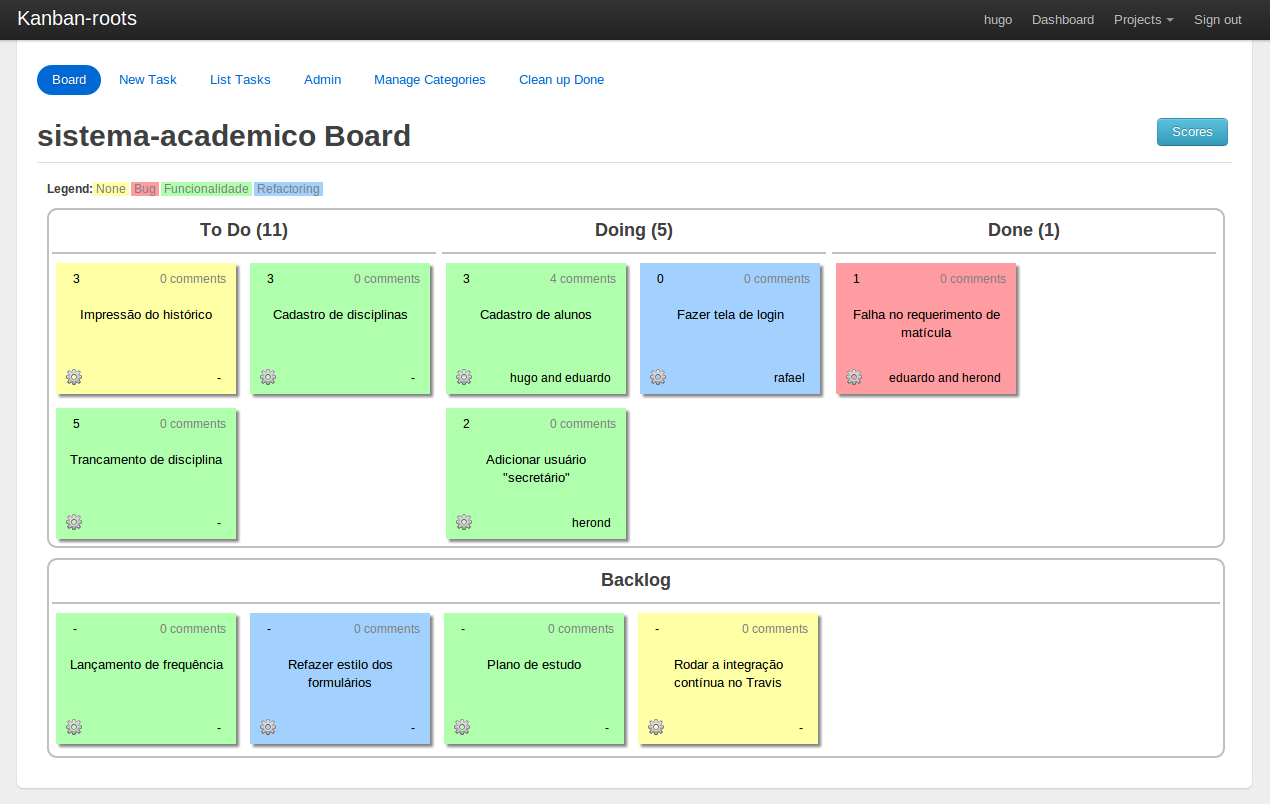
\includegraphics[scale=0.35]{images/kanban-roots}
  \label{img:tela_kaban_roots}
\end{figure}

\section{Contextualizando TDD}
\label{sec:contextualizando_tdd}

Para apresentar como a utilização do TDD se dá na prática, serão mostrados os passos para a implementação da seguinte funcionalidade chave para a montagem kanban:

\begin{quote}
\textit{Precisa-se saber todas as tarefas posicionadas em uma determinada posição do kanban (quadro) de um projeto.}
\end{quote}

A primeira coisa a ser feita é o teste para o caso mais simples: quando o projeto não tem tarefa alguma naquela determinada posição do kanban.

Desta forma, o teste de unidade para o caso mais simples pode ser como mostrado no código \ref{code:tdd_test1}, onde é criada uma instância da classe \texttt{Project} e é feita uma asserção de que não tem tarefas na posição ``\textit{Done}"\ do quadro.

\begin{mycode}{ruby}%
{Teste para o método Project\#tasks\_by\_position (versão 1)}{code:tdd_test1}
# test/unit/project_test.rb
class ProjectTest < ActiveSupport::TestCase
  def test_tasks_by_position
    project = Factory.create :project
    assert_equal(project.tasks_by_position("done"), [])
  end
end
\end{mycode}

Ao rodar este teste, ele irá falhar, informando que o método \texttt{tasks\_by\_position} sequer existe. Como esta era a falha esperada, é escrito então o código mais simples para passar neste teste, apresentado no código \ref{code:tdd_code1}, onde apenas é retornada uma lista vazia.

\begin{mycode}{ruby}%
{Implementação do método Project\#tasks\_by\_position (versão 1)}{code:tdd_code1}
# app/models/project.rb
def tasks_by_position position
  []
end
\end{mycode}

Os testes irão passar, mas a funcionalidade ainda não está completa e, consequentemente, o teste também não. Como pode ser visto no código \ref{code:tdd_test2}, é adicionado ao teste uma verificação de que para a posição 1 devem existir duas tarefas e que estas tarefas devem ser exatamente as criadas anteriormente.

\begin{mycode}{ruby}%
{Teste do método Project\#tasks\_by\_position (versão 2)}{code:tdd_test2}
# test/unit/project_test.rb
class ProjectTest < ActiveSupport::TestCase
  def test_tasks_by_position
    project = Factory.create :project
    tasks = [Factory.create(:task, :project => project, :position => "backlog"),
             Factory.create(:task, :project => project, :position => "backlog")]

    assert_equal(project.tasks_by_position("done"), [])

    assert_equal(project.tasks_by_position("backlog").count, 2)
    tasks.each { |task| assert(project.tasks_by_position("backlog").include?(task)) }
  end
end
\end{mycode}

Como o teste foi alterado, este é executado e irá falhar, informando que na \hyperref[code:tdd_test2]{linha 10} eram esperadas duas tarefas, mas foram obtidas zero. O código então deve ser modificado para passar no novo teste e é apresentado no código \ref{code:tdd_code2}.

\begin{mycode}{ruby}%
{Implementação do método Project\#tasks\_by\_position (versão 2)}{code:tdd_code2}
# app/models/project.rb
def tasks_by_position position
  task_list = []
  tasks.each do |task|
    task_list << task if task.position == position
  end
  task_list
end
\end{mycode}

Desta vez, após a modificação no código e a execução dos testes, todos os testes irão passar. Contudo, a cobertura de testes para este método ainda está fraca, o que pode ser resolvido com a adição de mais algumas tarefas em posições diferentes, como mostrado no código \ref{code:tdd_test3}.

\begin{mycode}{ruby}%
{Teste do método Project\#tasks\_by\_position (versão 3)}{code:tdd_test3}
# test/unit/project_test.rb
class ProjectTest < ActiveSupport::TestCase
  def test_tasks_by_position
    project = Factory.create :project
    tasks = [Factory.create(:task, :project => project, :position => "backlog"),
             Factory.create(:task, :project => project, :position => "backlog"),
             Factory.create(:task, :project => project, :position => "todo"),
             Factory.create(:task, :project => project, :position => "doing"),
             Factory.create(:task, :project => project, :position => "doing")]

    assert_equal(project.tasks_by_position("done"), [])

    assert_equal(project.tasks_by_position("backlog").count, 2)
    tasks[0..1].each { |task| assert(project.tasks_by_position("backlog").include?(task)) }

    assert_equal(project.tasks_by_position("todo"), [tasks[2]])

    assert_equal(project.tasks_by_position("doing").count, 2)
    tasks[3..4].each { |task| assert(project.tasks_by_position("doing").include?(task)) }
  end
end
\end{mycode}

Executando os testes novamente, todos eles passam, como mostrado na figura \ref{img:test-unit-exec}. Isto indica que já é hora de ir para o item 5 do ciclo TDD e refatorar. Ao comparar o código \ref{code:tdd_code2} com sua versão refatorada, apresentada no código \ref{code:tdd_code3}, pode-se perceber como a segunda está mais simples e clara e que ao rodar os testes, estes passam mostrando que o comportamento do método não mudou.

\begin{mycode}{ruby}%
{Implementação do método Project\#tasks\_by\_position (versão 3)}{code:tdd_code3}
# app/models/project.rb
def tasks_by_position position
  tasks.select { |item| item.position == position }
end
\end{mycode}

\begin{figure}[h]
  \center
  \caption{Saída produzida pela execução dos testes de unidade com utilizando TDD com testUnit}
  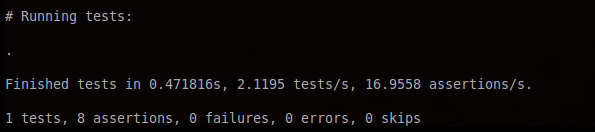
\includegraphics[scale=0.6]{images/test-unit-exec}
  \label{img:test-unit-exec}
\end{figure}

Com isso, o ciclo TDD para o desenvolvimento da funcionalidade é terminado, produzindo um código legível, limpo e bem coberto por testes, como pode ser visto no código \ref{code:tdd_code3}. Além disso, o código faz exatamente o que se espera dele, nada a mais nem nada a menos, atendendo os requisitos definidos nos testes, que são apresentados no código \ref{code:tdd_test3}.

Outro exemplo, neste caso de teste de integração, é o de uma extensão criada para fazer o destaque da sintaxe (\textit{highlighting}) de código na descrição das Tarefas e no conteúdo do Comentários no kanban-roots, como apresentado na figura \ref{img:highlighting}. Para isso, é utilizado um \textit{framework} em Python chamado Pygments\footnote{ Mais em \url{http://pygments.org/}}, que recebe como parâmetros uma \textit{string} com o código a ser destacado e a linguagem em que este código está escrito, retornando uma nova \texttt{string} em html com o código destacado.

\begin{figure}[h]
  \center
  \caption{Comentário com destaque da sintaxe de código no kanban-roots}
  \includegraphics[scale=0.5]{images/highlighting}
  \label{img:highlighting}
\end{figure}

O Pygments deve ser instalado na máquina onde o kanban-roots está sendo executado. No entanto, o kanban-roots foi projetado rodar tanto em um servidor próprio ou em um VPS\footnote{ \textit{Virtual Private Server}. É um servidor em ambiente compartilhado que possui acesso \textit{root} e processos independentes para cada conta VPS criada.}, como também no Heroku\footnote{ É um PaaS (\textit{platafom as a service}) que tem uma cota de utilização gratuita. No Heroku não é possível instalar dependências no sistema. Mais em \url{http://heroku.com}}. Sendo assim, além da possibilidade de utilizar o Pygments instalado localmente, foi utilizado um serviço gratuito e não oficial criado por Trevor Turk e hospedado no Google App Engine (GAE)\nomenclature{GAE}{Google App Engine} que permite a utilização da API \nomenclature{API}{Application programming interface} do Pygments através de uma requisição (através do método HTTP POST) para o serviço. \textbf{Dessa forma, deve-se testar a integração do kanban-roots com o Pygments instalado localmente e também com o serviço externo hospedado no GAE}.

Primeiramente, é feito o teste para o caso em que o Pygments é instalado localmente, apresentado no código \ref{code:integration_spec1}.

\begin{mycode}{rspec}%
{Teste de integração para o \textit{highlighting} de código (versão 1)}{code:integration_spec1}
# spec/lib/albino_render_spec.rb
describe HTMLwithAlbino do
  it "should get the highlighted block code from local pygments" do
    render = HTMLwithAlbino.new
    render.block_code('puts "hello!"', "ruby").should ==
      "<div class=\"highlight\"><pre>" +
        "<span class=\"nb\">puts</span> <span class=\"s2\">&quot;hello!&quot;</span>\n" +
      "</pre>\n</div>\n"
  end
end
\end{mycode}

A implementação para este teste é apresentado no código \ref{code:integration1}, onde o método \texttt{colorize} da classe \texttt{Albino} invoca o Pygments do sistema.

\begin{mycode}{ruby}%
{Implementação do \textit{highlighting} de código (versão 1)}{code:integration1}
# lib/albino_render.rb
class HTMLwithAlbino < Redcarpet::Render::HTML
  def block_code(code, lang)
    Albino.colorize(code, lang)
  end
end
\end{mycode}

Ao executar o teste, este passa. Como não tem nada para refatorar, é adicionado um novo teste para o caso em que o Pygments não está instalado no servidor, como é apresentado no código \ref{code:integration_spec2}.

É importante perceber que foi utilizado um dublê de teste (neste caso um \textit{stub}) para simular a resposta do método \texttt{can\_pygmentize?} que fará uma verificação no sistema operacional para identificar se o Pygments está instalado ou não.

\begin{mycode}{rspec}%
{Teste de integração para o \textit{highlighting} de código (versão 2)}{code:integration_spec2}
# spec/lib/albino_render_spec.rb
describe HTMLwithAlbino do
  it "should get the highlighted block code from local pygments" do
    @render.stub(:can_pygmentize?).and_return(true)
    render = HTMLwithAlbino.new
    render.block_code('puts "hello!"', "ruby").should ==
      "<div class=\"highlight\"><pre>" +
        "<span class=\"nb\">puts</span> <span class=\"s2\">&quot;hello!&quot;</span>\n" +
      "</pre>\n</div>\n"
  end

  it "should get the highlighted block code from pygments.appspot.com" do
    @render.stub(:can_pygmentize?).and_return(false)
    render = HTMLwithAlbino.new
    render.block_code('puts "hello!"', "ruby").should ==
      "<div class=\"highlight\"><pre>" +
        "<span class=\"nb\">puts</span> <span class=\"s2\">&quot;hello!&quot;</span>\n" +
      "</pre>\n</div>\n"
  end
end
\end{mycode}

O código \ref{code:integration2} apresenta a implementação que faz os dois casos de teste passarem. Nessa nova versão, foi preciso criar o método de suporte \texttt{can\_pygmentize?} que, como dito anteriormente, verifica se o Pygments está instalado. Se o Pygments estiver instalado, ele é invocado da mesma forma como na versão 1 da implementação. Porém, se o Pygments não estiver instalado, é feita uma requisição ao serviço externo.

\begin{mycode}{ruby}%
{Implementação do \textit{highlighting} de código (versão 2)}{code:integration2}
# lib/albino_render.rb
class HTMLwithAlbino < Redcarpet::Render::HTML
  def block_code(code, lang)
    if can_pygmentize?
      Albino.colorize(code, lang)
    else
      # This is a hack for pygments work on Heroku
      require "net/http"
      Net::HTTP.post_form(URI.parse("http://pygments.appspot.com/"),
                          {"code"=>code, "lang"=>lang}).body
    end
  end

  private
  def can_pygmentize?
    system "pygmentize -V"
  end
end
\end{mycode}

Como ao executar os testes, todos eles passam, podemos refatorar o código. Na implementação não há nada a ser refatorado, contudo, existe diversas duplicidades nos testes. O código \ref{code:integration_spec3} apresenta os testes refatorados, eliminando as duplicidades com a ajuda do método \texttt{before} que, ao receber o \texttt{:all} como parâmetro, é executado antes de de todos os casos de teste.

\begin{mycode}{rspec}%
{Teste de integração para o \textit{highlighting} de código (versão 3)}{code:integration_spec3}
# spec/lib/albino_render_spec.rb
describe HTMLwithAlbino do
  before(:all) do
    @render = HTMLwithAlbino.new
    @code_text = 'puts "hello!"'
    @highlighted_code =
      "<div class=\"highlight\"><pre>" +
        "<span class=\"nb\">puts</span> <span class=\"s2\">&quot;hello!&quot;</span>\n" +
      "</pre>\n</div>\n"
  end

  it "should get the highlighted block code from local pygments" do
    @render.stub(:can_pygmentize?).and_return(true)
    @render.block_code(@code_text, "ruby").should == @highlighted_code
  end

  it "should get the highlighted block code from pygments.appspot.com" do
    @render.stub(:can_pygmentize?).and_return(false)
    @render.block_code(@code_text, "ruby").should == @highlighted_code
  end
end
\end{mycode}

Desta forma, mostra-se que não apenas o código da implementação deve ser refatorado, mas também o código dos testes. Assim como o código da implementação, o código dos testes devem ser igualmente legíveis e otimizados, pois também sofrem manutenção e precisam ser executados com rapidez.

É importante lembrar que foram omitidos alguns casos de teste para esta funcionalidade, como por exemplo, o caso em que existe uma falha na requisição ao serviço externo. Esta omissão foi feita para que não o exemplo não ficasse muito extenso, e por este já cumprir seu objetivo.


\subsection{Design emergente no kanban-roots}
\label{sub:design_emergente_no_kanban_roots}

Para o desenvolvimento do kanban-roots, foi de extrema importância que o design evoluísse incrementalmente, pois não se sabia ao certo que
funcionalidades seriam contempladas nem que entidades existiriam.

As entidades \textit{Project} e \textit{Contributor} tinham uma relação direta, n para n, como apresentado na figura \ref{img:contributor_projetc}. Contudo, em um determinado momento achou-se pertinente a criação de uma nova entidade \textit{Team} que faria a ligação entre as outras duas entidades, como apresentado na figura \ref{img:contributor_team_projetc}. Isto acarretou uma série de alterações \cite{CommitAddTeam}, dentre outras, na interface das entidades e na estrutura do banco de dados $-$ considerada uma alteração crítica, mas que com ferramentas como \textit{migrations},\footnote{\textit{Migrations} são uma forma conveniente de gerenciar bases de dados de maneira estruturada e organizada. Mais em \url{http://guides.rubyonrails.org/migrations.html}} torna-se simples.

\begin{figure}[h]
  \center
  \caption{Diagrama de classes relacionando \textit{Contributor} e \textit{Project}}
  \includegraphics[scale=0.28]{images/contributor_projetc}
  \label{img:contributor_projetc}
\end{figure}

Meses depois, foi verificado que esta entidade \textit{Team} não era mais necessária, acarretando novamente em diversas modificações \cite{CommitRemoveTeam}, voltando ao estado apresentado na figura \ref{img:contributor_projetc}.

\begin{figure}[h]
  \center
  \caption{Diagrama de classes relacionando \textit{Contributor}, \textit{Team} e \textit{Project}}
  \includegraphics[scale=0.25]{images/contributor_team_projetc}
  \label{img:contributor_team_projetc}
\end{figure}

Foram diversas as situações em que mudanças como essa ocorreram durante o desenvolvimento do kanban-roots. Sem o suporte do TDD seria extremamente complicado fazer essas alterações e deixar o design emergir, pois a insegurança de que as modificações pudesse afetar outras partes do código seria muito grande. Além disso, a criação a priori dos testes favoreceu que as modificações fossem feitas de maneira mais simples, direta e rápida.

\subsection{A ubiquidade do TDD}
\label{sub:a_ubiquidade_do_tdd}

Existe uma controvérsia sobre a não utilização do TDD em qualquer situação. É dito ``sobre a \textbf{não} utilização"\ pois o autor do presente trabalho desconhece qualquer literatura dizendo que TDD deve ser utilizado sempre e em qualquer situação. Porém, muitos defendem a sua não utilização em algumas situações como em fase de descobertas, em fase de experimentos, se o desenvolvedor nunca utilizou a API, se o código não será utilizado novamente ou se levar mais tempo para escrever os testes do que para escrever e executar o código.

\citeonline{CleanCode} define As Três Leis do TDD, onde a primeira delas é: ``Você não pode escrever código de produção até que você tenha escrito um teste de unidade com falha.". Deve-se ter bastante atenção para o trecho ``de produção", pois sem ele, o sentido da frase é completamente distorcido, dando a impressão de que deve-se utilizar em todas as situações.

Introduzindo o kanban-roots na discussão, nos dois únicos casos em que ocorreu um \textit{bug} em produção, ao ser feita uma analise no código em busca da solução, foi encontrado um comentário ``TODO: Make test and refactor"\ nos métodos onde os \textit{bugs} ocorreram. Atualmente, existem 5 comentários semelhantes a esse espalhados no código do kanban-roots. Isso, de certa forma, comprova que caso os testes não sejam escritos antes, para um código que irá entrar em produção, escrevê-lo depois acaba sendo um fardo, e isso é ignorado até que um problema ocorra.

Um exemplo para esta situação é apresentado no código \ref{code:todo}, onde é mostrado um método de \textit{controller}\footnote{O \textit{controller} é um componente do padrão MVC (do inglês \textit{Model View Controller}) de desenvolvimento de software. Neste padrão, a lógica da aplicação (\textit{Model}) é isolada da interface do usuário (\textit{View}) através de um controlador (\textit{Controller}).} que é chamado via Ajax e implementa a atualização dos pontos de uma tarefa diretamente do kanban do projeto. Além de atualizar os pontos da tarefa na base de dados, este método captura, trata e envia informações para que a interface do kanban seja atualizada. Este foi um típico caso onde um experimento foi para produção, sem testes e com um código \textbf{extremamente ruim}.

\newpage

\begin{mycode}{ruby}%
{Código do método que atualiza os pontos de uma tarefa diretamente do kanban do projeto}{code:todo}
# app/controllers/boards_controller.rb
class BoardsController < InheritedResources::Base
  # TODO: Make test and refactor
  def update_points
    task = Task.find(params[:task_id])
    points = params[:points] == '-' ? nil : params[:points]

    position = Board::POSITIONS.key(task.position)
    if position != 'done'
      score = 0
    else
      if task.points.nil?
        old_points = 0
      elsif task.points.zero?
        old_points = 0.1
      else
        old_points = task.points
      end
      if points.nil?
        new_points = 0
      elsif points.to_i.zero?
        new_points = 0.1
      else
        new_points = points.to_i
      end
      score = new_points - old_points
    end

    task.update_attribute(:points, points)

    project = Project.find(task.project_id)
    division_name = Board::POSITIONS[params[:division_id]]
    division_points = project.count_points(division_name)
    contributors = task.contributor_ids
    data = { :division_points => division_points,
             :contributors => contributors,
             :score => score }
    render :text => data.to_json
  end
end
\end{mycode}

Códigos como o apresentado acima são extremamente difíceis de serem testados, pois, além de possuir complexidade ciclomática\footnote{Complexidade ciclomática (ou complexidade condicional) é uma métrica de software usada para indicar a complexidade de um programa de computador. Ela mede a quantidade de caminhos de execução independentes a partir de um código fonte.} acima do aceitável, desempenham tarefas de responsabilidade de outras unidades do software, o que aumenta em muito o seu acoplamento e dificulta a escrita dos testes. Se este código fosse escrito utilizando TDD, certamente estaria melhor escrito e com mais qualidade, pois para escrever o teste, o código teria que ser refatorado de modo a distribuir as diferentes responsabilidades incorporadas no mesmo. Assim, fica clara a íntima relação entre teste e implementação no que tange ao design e à qualidade.

\citeonline{LegacyCode} define que \textbf{código legado é código sem testes}. Esta afirmação, que pode parecer extremada, é simplesmente a constatação de que, sem uma ampla cobertura de testes automatizados, e uma vez que é economicamente inviável a aplicação manual de todos os casos de teste $-$ ou mesmo de parte deles $-$ de um software a cada modificação, é muito difícil ter uma margem razoável de segurança de que uma modificação não irá introduzir \textit{bugs} no software. Deste modo, para um código ``que irá para produção"\ a utilização do TDD é essencial, pois do contrário, se está criando código legado. É importante lembrar que o código legado com o tempo vai minando a manutenibilidade do sistema e assim, elevando os custos de introdução de novas funcionalidade e evolução do mesmo.

Conclui-se que, para quem adota TDD, somente nos casos em que um código será posteriormente eliminado, como em provas de conceito temporárias ou experimentos, a utilização da técnica não é invariavelmente necessária. Contudo, a utilização de TDD nesses cenários pode ser muito interessante, pois como dito anteriormente, para a escrita dos testes, é preciso entender bem o problema a ser resolvido, fazendo o desenvolvedor se preparar mais para o que ele ainda não conhece muito bem.


\section{Contextualizando BDD}

Nesta seção será visto como se dá a utilização do BDD se dá na prática, bem como sua relação com TDD, além de uma discussão acerca dos modelos de escrita dos testes com a utilização desta técnica.

\subsection{A relação entre BDD e TDD}
\label{sub:a_relacao_entre_bdd_e_tdd}

Como dito a anteriormente, BDD é uma evolução do TDD. A grande diferença entre os dois é que TDD não abrange a validação do software, ou seja, se o software atende os requisitos. Isso muda tudo, pois em BDD, a ênfase está no comportamento, e não na estrutura. Ao invés de focar em classes e métodos ao escrever os testes, o foco é no comportamento que gera valor para o sistema. Além disso, o pensamento não é voltado à verificação, mas sim no comportamento, em validar que o software faz sem deixar também de verificar se está funcionando como deveria.

Em BDD não são escritos testes, mas sim especificações, chamadas de \textit{specs} (de \textit{specifications}). Pode-se ter a clara diferença entre testes (TDD) e specs (BDD) comparando o código \ref{code:tdd_test3} com o código \ref{code:bdd_spec}, onde palavras chave como \textit{class}, \textit{test} e \textit{assert} dão lugar a \textit{describe}, \textit{it} e \textit{should}, ficando nítido o foco no comportamento. Além disso, a substituição do Test::Unit (TDD) pelo Rspec (BDD) também revela grande mudança nas asserções onde os \textit{asserts} dão lugar aos \textit{matchers}, fazendo com que as asserções possam ser lidas quase como uma linguagem natural.

\begin{mycode}{rspec}%
{Exemplo de uma spec}{code:bdd_spec}
# spec/models/project.rb
describe Project do
  it "returns all related tasks matching a given position" do
    project = Factory.create :project
    tasks = [Factory.create(:task, :project => project, :position => 1),
             Factory.create(:task, :project => project, :position => 1),
             Factory.create(:task, :project => project, :position => 2),
             Factory.create(:task, :project => project, :position => 3),
             Factory.create(:task, :project => project, :position => 3)]

    project.tasks_by_position(4).should be_empty

    project.should have(2).tasks_by_position(1)
    project.tasks_by_position(1).should include(*tasks[0..1])

    project.tasks_by_position(2).should == [tasks[2]]

    project.should have(2).tasks_by_position(3)
    project.tasks_by_position(3).should include(*tasks[3..4])
  end
end
\end{mycode}

Em TDD, o nome dos testes é baseado na estrutura do código, e isso pode ter um efeito colateral: criar duplicações. Ao escrever testes como o \texttt{test\_tesks\_by\_position} do código \ref{code:tdd_test3} e o método \texttt{tasks\_by\_position} é renomeado, o nome do teste também terá que ser renomeado, o que na maioria das vezes é esquecido. Isso torna os testes confusos e desinformativos \cite{ContinuousTesting}. Como por definição, refatorar é melhorar a estrutura e o design do código sem alterar seu comportamento, nomeando os testes com base no comportamento desejado ao invés da estrutura do código, não apenas torna os testes mais informativos como também torna a refatoração menos custosa \cite{ContinuousTesting}.

% subsection a_relacao_entre_bdd_e_tdd (end)


\subsection{Modelos de escrita dos testes de aceitação}
\label{sub:modelos_de_escrita_dos_testes_de_aceitacao}

Existem duas maneiras principais de se escrever os testes de aceitação: em texto plano e em código puro. Para exemplificar cada uma das abordagens, será especificada a seguinte funcionalidade:

\begin{quote}
\textit{Os comentários mostrados na página de tarefas devem ser renderizados utilizando a linguagem de marcação Markdown.}
\end{quote}

O resultado desta funcionalidade implementada é apresentado na figura \ref{img:markdown}.

\begin{figure}[h]
  \center
  \caption{Comentários renderizados com Markdown no kanban-roots}
  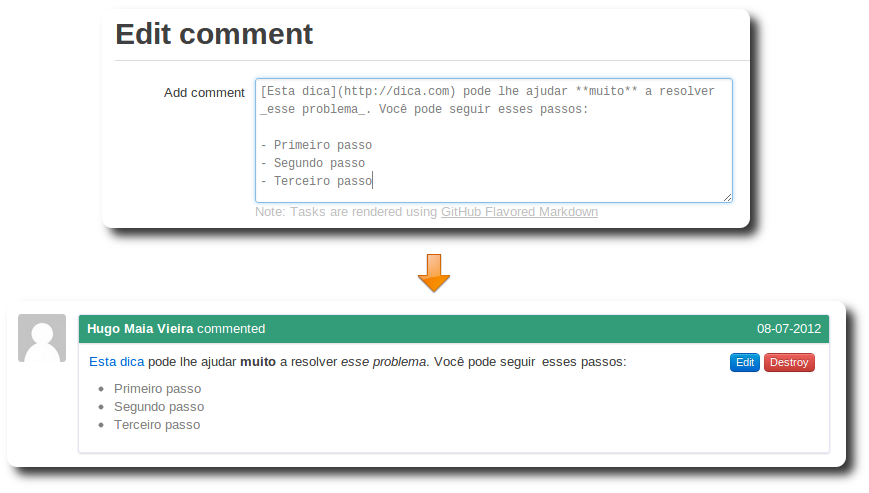
\includegraphics[scale=0.5]{images/markdown}
  \label{img:markdown}
\end{figure}

\subsubsection{Escrita em texto plano}
\label{ssub:escrita_em_texto_plano}

Uma das maneiras de escrever testes de aceitação é como texto plano, em uma linguagem natural, ou seja, inglês, português e etc.

\citeonline{IntroducingBDD} estabelece um \textit{template} para a escrita para este tipo de especificação, sendo este uma captura dos critérios de aceitação de uma história:

\begin{quote}
\textbf{As a} (Como um) [X]\\
\textbf{I want} (Eu quero) [Y]\\
\textbf{So that} (Para que) [Z]
\end{quote}

Onde Y é uma funcionalidade, Z é o benefício ou valor da funcionalidade e X é a pessoa (ou regra) que irá se beneficiar desta funcionalidade. O mapeamento feito desta forma é interessante pois se não souber completar Z, isso quer dizer que esta funcionalidade pode não ser tão importante quanto se imaginava.

Para finalizar esse \textit{template}, os critérios de aceitação da história são quebrados em diferentes cenários que tem a seguinte forma:

\begin{quote}
\textbf{Given} (Dado) algum contexto inicial\\
\textbf{When} (Quando) algum evento ocorre\\
\textbf{Then} (Então) certifique-se de alguns resultados
\end{quote}

Nas ferramentas que implementam esta abordagem, os testes são escritos baseados em \textit{steps} (passos), onde cada \textit{step} (Given/When/Then) é mapeado para um código real.

No código \ref{code:bdd_cucumber_spec}, é utilizado o \textit{Cucumber} para fazer a especificação. Como pode-se ver, o teste é escrito em uma linguagem que qualquer pessoa, mesmo sem nenhum conhecimento em programação, pode ler e validar.

\begin{mycode}{cucumber}%
{Especificação em texto plano}{code:bdd_cucumber_spec}
# features/comments.feature
Feature: Render comments with Markdown syntax
  As a user
  I want to use Markdown in my comments
  In order to make my comments more expressives

  Scenario: on tasks page
    Given I am a contributor of "sgtran" project
    And I am authenticated
    And I have a task of "sgtran" project
    When I am on the task page
    And I fill in "comment_content" with "# Some content [link](http://exemplo.com)"
    And I press "Comment"
    Then I should see "Some content" in a "h1" tag
    And I should see "link" in an "a" tag
\end{mycode}

Para cada \textit{step} existe uma implementação, ou seja, sua definição, chamada de \textit{step definition}. Pode-se pensar nos \textit{steps} como chamadas à métodos, e assim, os \textit{step definitions} serão as definição desses métodos. Deste modo, ao rodar os testes, o arquivo de teste é parseado e os \textit{steps} são executados.

Os \textit{step definitions} para os \textit{steps} do código \ref{code:bdd_cucumber_spec} são apresentado no código \ref{code:step_definition}. Como durante o desenvolvimento são escritos muitos \textit{step definitions}, com o intuito de organizá-los, eles são separados por contexto em diferentes arquivos.

\begin{mycode}{ruby}%
{Step definitions}{code:step_definition}
# features/step_definitions/contributor_steps.rb
Given /^I am a contributor of "([^"]*)" project$/ do |name|
  @project = Factory.create :project, :name => name
  @contributor = Factory.create :contributor, :contributions => [@project]
  @project.update_attribute(:contributors, [@contributor])
end

# features/step_definitions/contributor_steps.rb
Given /^I am(?:| an) authenticated(?:| contributor)$/ do
  @contributor ||= Factory.create :contributor

  Given %{I am on the sign in page}
  And %{I fill in "contributor_login" with "#{@contributor.email}"}
  And %{I fill in "contributor_password" with "#{@contributor.password}"}
  And %{I press "Sign in"}
end

# features/step_definitions/task_steps.rb
Given /^I have a task of "([^"]*)" project$/ do |project_name|
  @project = Factory.create :project, :name => 'project_name'
  @task = Factory.create :task, :project => @project, :author => @contributor
end

# features/step_definitions/web_steps.rb
Given /^(?:|I )am on (.+)$/ do |page_name|
  visit path_to(page_name)
end

# features/step_definitions/web_steps.rb
When /^(?:|I )fill in "([^"]*)" with "([^"]*)"$/ do |field, value|
  fill_in(field, :with => value)
end

# features/step_definitions/web_steps.rb
When /^(?:|I )press "([^"]*)"$/ do |button|
  click_button(button)
end

# features/step_definitions/my_web_steps.rb
When /^I should see "([^"]*)" in a(?:|n) "([^"]*)" tag$/ do |text, tag|
  if page.respond_to? :should
    page.should have_xpath("//#{tag}", :text => text)
  else
    assert page.has_xpath?("//#{tag}", :text => text)
  end
end
\end{mycode}

Na figura \ref{img:cucumber-exec} é apresentada a saída para a execução do teste. Ao lado de cada passo, é mostrado em que arquivo este passo está definido, com o objetivo de facilitar em momentos onde se deseja depurar os erros. Pode-se perceber que neste caso simples, existem cinco arquivos diferentes envolvidos no teste.

\begin{figure}[h]
  \center
  \caption{Saída produzida pela execução dos testes utilizando escrita em texto plano com o Cucumber}
  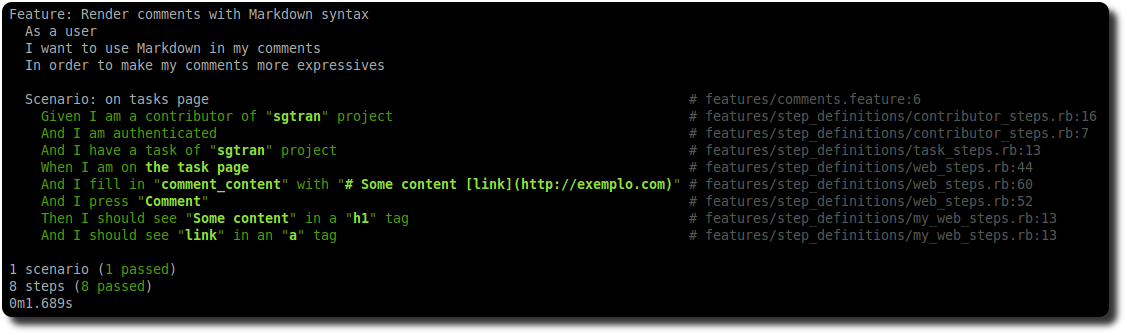
\includegraphics[scale=0.4]{images/cucumber-exec}
  \label{img:cucumber-exec}
\end{figure}


\subsubsection{Escrita em código puro}
\label{ssub:Escrita em codigo puro}

A outra maneira de escrever os testes de aceitação é com código puro. Nesta forma, todo o código dos testes (descrição e implementação) está concentrado em apenas um lugar, utilizando somente código para escrever os testes.

No código \ref{code:bdd_spec1} pode-se ver a especificação em código puro para a funcionalidade.

\begin{mycode}{rspec}%
{Especificação em código puro}{code:bdd_spec1}
# spec/acceptance/comments_spec.rb
feature "Render comments with Markdown syntax" do
  background do
    @owner = Factory.create :contributor
    @project = Factory.create :project
    @task = Factory.create :task, :project => @project, :author => @owner
    login(@owner.email, @owner.password)
  end

  scenario "on tasks page" do
    visit project_task_path(@project, @task)
    fill_in "comment_content", :with => "# Some content [link](http://exemplo.com)"
    click_button "Comment"
    page.should have_xpath("//h1", :text => "Some content")
    page.should have_xpath("//a", :text => "link", :href => "http://exemplo.com")
  end
end
\end{mycode}

É importante ressaltar que, mesmo sem a utilização dos \textit{templates} de história e cenário, este modelo de escrita não deixa de ser BDD \cite{BDDSolis}, pois o foco da escrita dos testes continua no comportamento.

Na figura \ref{img:rspec-acceptance-exec} é apresentada a saída para a execução do teste. Neste caso, um único arquivo concentra tudo relativo ao teste.

\begin{figure}[h]
  \center
  \caption{Saída produzida pela execução dos testes utilizando escrita em código puro com RSpec + Capybara}
  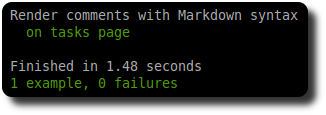
\includegraphics[scale=0.6]{images/rspec-acceptance-exec}
  \label{img:rspec-acceptance-exec}
\end{figure}


\subsubsection{Pontos em aberto sobre os modelos de escrita}
\label{ssub:pontos_em_aberto}

BDD vem se tornando um consenso em automação de testes. Contudo, existem uma divergência grande sobre a forma de escrita dos testes de aceitação entre escrita em código puro e escrita em texto plano, tendo alguns pontos a serem considerados.


\paragraph{Legibilidade}
\label{sssub:legibilidade}

Muitos defendem que os testes devem ser escritos em texto plano, por conta do teste ser escrito em linguagem que qualquer pessoa, mesmo sem nenhum conhecimento em programação, pode ler e validar.

Em uma situação onde se está desenvolvendo uma aplicação para um cliente, existe um mito sobre o cliente escrever as especificações, contudo está é uma abordagem utópica \cite{SteakOverCucumber, CucumberForVegetarians, ClientsWritingCucumber}. O cliente pode até ler e validar $-$ o que segundo \citeonline{YankoCapybara} nunca acontece $-$ mas mesmo assim esta não é uma abordagem muito interessante.

O cliente é especialista em problemas e os desenvolvedores em dar soluções. Se o cliente escreve a especificação, na realidade ele está escrevendo parte da solução \cite{SteakOverCucumber}. No caso da funcionalidade exemplificada anteriormente, o cliente apenas sabe que os ``comentários devem ser renderizados com markdown", ele não quer saber se para isso deve entrar em determinada página, preencher determinado campo e clicar em determinado botão. O cliente apenas sabe a funcionalidade que ele deseja, e vê-la funcionando.

Dessa forma, o cliente não tem interesse em ler a especificação como no código \ref{code:bdd_cucumber_spec}, nem validá-la, muito menos escrevê-la. Ler somente ``Render comments with Markdown syntax" é o suficiente, mais do que isso é superficial \cite{WhyBotherWithCucumberTesting}. Os testes em texto plano se atem a detalhes de interface que são irrelevantes para os objetivos do cliente.

Uma exceção a isto ocorre em áreas que fazem uso pesado de modelagem de processo de negócio (BPM, do inglês \textit{Business Process Modeling}) \nomenclature{BPM}{Business Process Modeling} como Enterprise Information Systems, na qual descrições executáveis em texto plano podem servir como ligação entre os artefatos de BPM e o código executável, sendo, neste caso, uma forma de explicitar critérios de aceitação. \cite{IntroducingBLDD}.

Já em um contexto como o do desenvolvimento do kanban-roots, no qual não existe um cliente, onde as pessoas que escrevem e leem as especificações são desenvolvedores, a escrita em texto plano tem um valor ainda menor. O código é uma linguagem natural para desenvolvedores, ainda mais quando é escrito em conjunto com DSLs\footnote{\textit{Domain specific language} (linguagem específica de domínio) é uma linguagem de programação de expressividade limitada, focada num domínio particular.} \nomenclature{DSL}{Domain specific language} como a do Rspec \cite{SteakOverCucumber}.


\paragraph{Camada adicional}
\label{sssub:camada_adicional}

Outra crítica aos testes em texto plano é que enquanto nos testes em código puro todo o código do teste está em concentrado em apenas um lugar, nos testes em texto plano, o código do testes está espalhado em diversos arquivos e métodos, devido a camada adicional dos \textit{steps}, tonando a suíte de testes mais complexa de manter e estender \cite{SteakOverCucumber}.

Além disso, é necessário manter um segundo ambiente de testes, já que para escrever os testes de aceitação em texto plano é necessária uma ferramenta de testes específica para isso. Isso não acontece com a escrita em código puro, já que é utilizada a mesma ferramenta utilizada nos testes unitários \cite{WhyBotherWithCucumberTesting}.


\paragraph{Tempo de execução}
\label{sssub:tempo_de_execucao}

Outro questionamento é sobre a velocidade para a execução dos testes. Como o \textit{Cucumber} utiliza a \textit{Gherkin}\footnote{\url{http://github.com/cucumber/cucumber/wiki/Gherkin}}, que é uma DSL externa\footnote{Uma DSL que tem sua própria sintaxe e necessita de um \textit{parser} para processá-la \cite{DSLFowler}.}, o arquivo de \textit{features} é parseado para que os \textit{steps} sejam executados, introduzindo um tempo extra na execução dos testes.

Para um conjunto de funcionalidades, foram escritos testes utilizando os ambos modelos de escrita $-$ apresentados no Anexo \ref{cha:codigo_do_comparativo}. Cada conjunto de vinte e dois exemplos foi executado separadamente e seus tempos de execução medidos, sendo os resultados apresentados na tabela \ref{table:tempo_de_execucao}.

\begin{table}[ht]
\caption{Velocidade de execução dos testes de acordo com o método de escrita}
\label{table:tempo_de_execucao}
\centering
\begin{tabular}{p{4.5cm} p{6.5cm}}
\toprule
\textbf{Método de escrita} & \textbf{Tempo médio de execução} \\
\midrule[1pt]
texto plano & 0m11.667s \\ \midrule
código puro & 0m8.8385s \\
\bottomrule
\end{tabular}
\end{table}

Analisando estes resultados pode-se concluir que os testes em código puro executam, em média, em um tempo 25\% menor que os em texto plano.


\subsubsection{Um modelo híbrido de escrita}
\label{ssub:um_modelo_hibrido_de_escrita}

\citeonline{YankoCapybara} apresenta um modelo alternativo de escrita de testes de aceitação, sendo esta uma união entre os duas maneiras apresentadas anteriormente\footnote{Esta abordagem também é utilizada pelo \textit{framework} easyb para Java. Mais em \url{http://www.easyb.org}}. Os testes são escritos em código puro, porém utilizando \textit{steps} semelhantes aos do testes em texto plano. No código \ref{code:rspec_steps} é apresentado o exemplo anterior utilizando este novo modelo\footnote{Para a escrita deste exemplo, foi utilizada uma ferramenta criada por Yanko chamada \textit{Rspec example steps}. Mais em \url{https://github.com/railsware/rspec-example_steps}}.

\begin{mycode}{rspec}%
{Especificação mesclando código puro com texto plano}{code:rspec_steps}
feature "Render comments with Markdown syntax" do
  background do
    @owner = Factory.create :contributor
    @project = Factory.create :project
    @task = Factory.create :task, :project => @project, :author => @owner
    login(@owner.email, @owner.password)
  end

  Steps "Render on tasks page" do
    When "I am on the task page" do
      visit project_task_path(@project, @task)
    end
    And "I fill in the comment with an text with markdown syntax" do
      fill_in "comment_content", :with => "# Some content [link](http://exemplo.com)"
    end
    And "I press the Comment buttom" do
      click_button "Comment"
    end
    Then "I should see the text rendered as HTML" do
      page.should have_xpath("//h1", :text => "Some content")
      page.should have_xpath("//a", :text => "link", :href => "http://exemplo.com")
    end
  end
end
\end{mycode}

Esta abordagem busca eliminar os problemas com a camada adicional e tempo de execução que a escrita em texto plano têm. Além disso, busca também aprimorar legibilidade da documentação da escrita em código puro, pois os testes, ao serem executados, produzem uma saída como mostrado na figura \ref{img:output-novo-modelo}

\begin{figure}[h]
  \center
  \caption{Saída produzida pela execução dos testes utilizando modelo proposto por Yanko}
  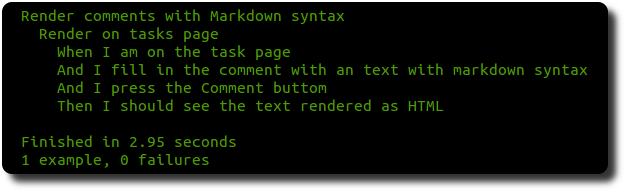
\includegraphics[scale=0.6]{images/output-novo-modelo}
  \label{img:output-novo-modelo}
\end{figure}

No entanto, esta abordagem cai no mesmo dilema da escrita em texto plano: o cliente não irá ler ou validar esta saída. Além disso, a introdução dos métodos \texttt{When/And/Then} juntamente com as \textit{strings} e blocos passados como parâmetros, piora muito a legibilidade do código de teste, prejudicando a manutenibilidade da suíte de testes. Assim, está abordagem, apesar de eliminar a camada adicional, pouco difere da escrita em texto plano, no que diz respeito às desvantagens.


\subsubsection{Reflexões acerca do modelo de escrita}
\label{ssub:reflexoes_bdd}

Analisando o exposto anteriormente, pode-se perceber os testes escritos em texto plano em um primeiro momento são muito atraentes, pois, com a facilidade de leitura, a possibilidade de validação de testes executáveis pelo cliente se tornam reais. No entanto, como apresentado anteriormente, na realidade é pouquíssimo provável que o cliente irá validar estes testes. Isto é ainda mais acentuado em projetos como o kanban-roots onde não existe cliente em si, tornando praticamente irrelevante os possíveis benefícios da escrita de testes em texto plano.

Já para projetos grandes, nos quais a suíte de testes é extensa, 25\% a mais no tempo de execução dos testes é um preço alto a ser pago, pois os testes devem ser executados diversas vezes ao dia. Se o tempo necessário para executar a suíte de testes se tornar demasiadamente longo, o desenvolvedor tende a rodar os testes menos vezes, diminuindo, assim, a eficácia da aplicação do BDD. Além disso, a escrita de testes em texto plano prejudica a produtividade, pois é adicionada complexidade ao processo, devido à camada adicional, fazendo com que a produtividade seja reduzida.

Apesar dos pontos negativos, os testes em texto plano podem ter valia em situações onde o desenvolvedor tem grandes dificuldades em entender o que o cliente quer ou entender o um determinado processo realizado pelo cliente. Desta forma, o teste em texto plano pode servir como um facilitador na comunicação. Assim, sentados lado a lado, o cliente vai dizendo ao desenvolvedor qual é o fluxo, e o desenvolvedor por sua vez, vai mapeando para o teste. Como ambos conseguem ler e entender o que está sendo escrito, a discussão e entendimento do problema é facilitada.


\section{Contextualizando Integração contínua}

Nesta seção será feita uma discussão acerca das características das integrações síncrona e assíncrona, além de mostrar como a integração contínua foi feita no kanban-roots.

\subsection{Integração contínua síncrona versus assíncrona}
\label{sub:sincrona_x_assincrona}

Sempre que possível, o melhor modelo de integração a ser utilizado é o síncrono. Pode-se fazer essa afirmação baseado no que \citeonline{ArtOfAgileDevelopment} descrevem como vantagens em utilizar a integração contínua síncrona:

\begin{itemize}
  \item Se a \textit{build} falhar, não é necessário interromper uma nova tarefa iniciada para voltar e corrigir a anterior, evitando assim a mudança de contexto mental.
  \item Ajuda a manter a \textit{build} rápida, pois se está levando muito tempo para executar, a percepção é imediata e pode ser logo corrigida.
  \item A frequência de \textit{builds} quebradas é muito menor, assim o tempo de permanência da falha no sistema de controle de versão, pois o responsável pela modificação que introduziu a falha pode não estar apto para corrigir-la imediatamente.
\end{itemize}

\citeonline{ImproveitCI} corrobora dizendo que a integração contínua assíncrona permite o trabalho de desenvolvedores distribuídos geograficamente, porém é um pouco mais arriscada e menos eficiente que a integração síncrona. O risco aumenta porque o repositório pode ficar inconsistente durante alguns períodos de tempo $-$ sempre que um erro ocorre e o responsável por ele ainda não fez o \textit{commit} das correções. Na integração assíncrona, a eficiência diminui porque leva mais tempo para o desenvolvedor descobrir que cometeu um erro. É comum o desenvolvedor receber a notificação de um erro depois de já ter iniciado uma nova atividade. Ao ser notificado, deve parar a nova tarefa, relembrar o que havia feito na tarefa anteriormente e corrigir o erro. O processo síncrono é mais eficiente no uso do \textit{feedback} exatamente porque impede o desenvolvedor de desviar sua atenção para qualquer outra atividade, enquanto a integração não tiver sido concluída com sucesso.


\subsection{Integração contínua no kanban-roots}
\label{sub:integracao_continua_no_kanban}

Com base no tópico anterior e por ser um projeto \textit{open source}, no kanban-roots foi utilizado o método assíncrono de integração contínua, através do Travis\footnote{Mais informações podem ser encontradas em \url{http://travis-ci.org}}, que foi escolhido por ser um serviço hospedado e gratuito de integração contínua para a comunidade \textit{open source}, o que facilitou bastante pela não necessidade de manutenção de uma estrutura local de integração contínua. Na figura \ref{img:travis-success} é apresentada a tela do Travis quando a \textit{build} é executada com sucesso e na figura \ref{img:travis-fail} quando a \textit{build} falha.

\begin{figure}[h]
  \center
  \caption{Tela do Travis quando a \textit{build} é executada com sucesso}
  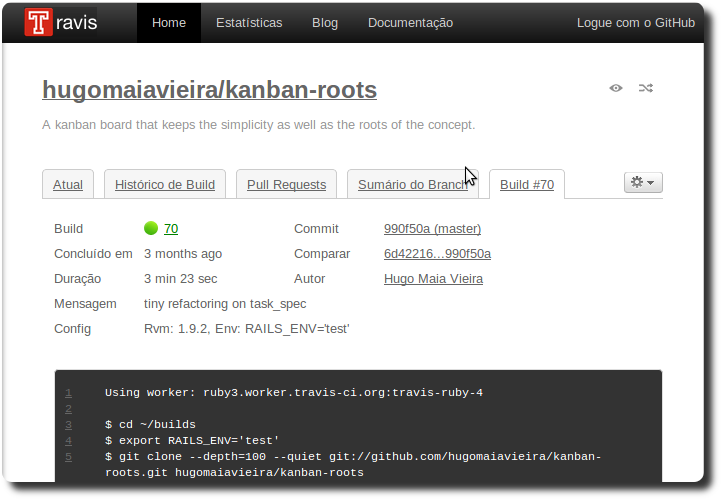
\includegraphics[scale=0.55]{images/travis-success}
  \label{img:travis-success}
\end{figure}

Na Seção \ref{sec:contextualizando_tdd} sobre testes de integração, foi apresentado o código \ref{code:integration_spec3} com os testes de integração para o \textit{highlighting} de código. Para que a integração contínua pudesse continuar sendo executada no Travis, o teste que verifica a integração do kaban-roots com o Pygments local foi comentado, uma vez que não é possível fazer instalações de dependências de sistema no Travis. Neste caso, o ideal seria ter um servidor próprio para rodar a integração contínua, pois esta tem que simular um ambiente de produção da forma mais perfeita possível, utilizando o Jenkins\footnote{Mais informações em \url{http://jenkins-ci.org/}} por exemplo.

\begin{figure}[h]
  \center
  \caption{Tela do Travis quando a \textit{build} falha}
  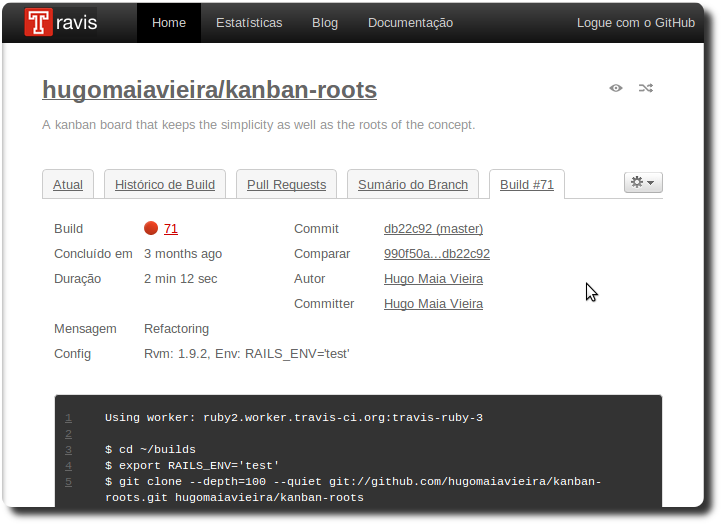
\includegraphics[scale=0.55]{images/travis-fail}
  \label{img:travis-fail}
\end{figure}

A integração contínua se mostrou importante em algumas ocasiões durante o desenvolvimento do kanban-roots, a exemplo:

\begin{itemize}
  \item Alguns arquivos não foram incluídos no \textit{commit}, fazendo com que localmente tudo funcionasse perfeitamente, mas o repositório estava quebrado.
  \item Em ambiente de desenvolvimento é utilizado o SQLite\footnote{\url{http://www.sqlite.org}} e em ambiente de produção, é utilizado o MySQL\footnote{\url{http://www.mysql.com}}. Assim, foi feita uma \textit{query} que apenas funcionava no SQLite, mas não no MySQL. Ou seja, em desenvolvimento estava perfeito, mas em produção, não.
\end{itemize}

Com o \textit{feedback} rápido da integração contínua, todas as falhas foram corrigidas muito rapidamente, sem que problemas maiores ocorressem e outras modificações na base de código fossem feitas sobre as modificações problemáticas, o que faria com que a correção dos problemas fosse mais complexa e levasse mais tempo.


\section{Contextualizando dublês de teste}

Nesta seção será feita a contextualização dos dublês de teste \textit{stub} e \textit{mock}, com exemplos de utilização no kanban-roots. Além disso, será feita uma discussão sobre a dicotomia entre o TDD clássico e o mockista.

\subsection{Contextualizando o \textit{stub}}
\label{sub:contextualizando_o_stub}

Um exemplo da utilização simples e eficiente do \textit{stub} foi mostrado no teste de integração apresentado na Seção \ref{sec:contextualizando_tdd}. Naquele exemplo, foi feito um \textit{stub} do método \texttt{can\_pygmentize?} que faz uma consulta ao sistema operacional para verificar se uma determinada dependência de sistema está instalada. Desta forma, o teste ficou isolado, não importando se a máquina em que o teste for executado tem ou não a dependência instalada, sendo assim possível simular as duas situações $-$ logicamente, uma maquina não pode, ao mesmo tempo, ter e não ter uma dependência instalada.

Um outro exemplo é mostrado no código \ref{code:stub_spec}, onde está sendo testada uma ação da classe \textit{Project}. Contudo, para que esta ação seja realizada, é necessário um conjunto de objetos da classe \textit{Task}. Assim, com o objetivo de criar um teste isolado e concentrado na classe \textit{Project}, é utilizado o método \texttt{stub\_model} que cria um \textit{stub} da classe \textit{Task} que irá reponder apenas aos atributos definidos no \textit{hash} passado como segundo parâmetro. No caso, a ação em questão é contar a soma dos pontos das tarefas alocadas em uma determinada posição do quadro (kanban). Esta ação é exercida através do método \texttt{count\_points}, cuja implementação é apresentada no código \ref{code:stub}. Na figura \ref{img:count-points} é apresentada uma utilização do método \texttt{count\_points} no somatório de pontos das tarefas na posição \textit{To Do} do kanban.

\begin{mycode}{rspec}%
{Exemplo do \textit{stub} da classe \textit{Task}}{code:stub_spec}
# spec/models/project_spec.rb
describe Project do
  it "returns the tasks points sum for a given position of the board" do
    tasks = [stub_model(Task, :points => 1, :position => Board::POSITIONS["doing"]),
             stub_model(Task, :points => 2, :position => Board::POSITIONS["doing"]),
             stub_model(Task, :points => 8, :position => Board::POSITIONS["todo"]),
             stub_model(Task, :points => nil, :position => Board::POSITIONS["todo"]),
             stub_model(Task, :points => 3, :position => Board::POSITIONS["doing"]),
             stub_model(Task, :points => 5, :position => Board::POSITIONS["todo"])]
    project = Project.new
    project.tasks.<<(*tasks)

    project.count_points(Board::POSITIONS["todo"]).should == 13
    project.count_points(Board::POSITIONS["doing"]).should == 6
    project.count_points(Board::POSITIONS["done"]).should == 0
  end
end
\end{mycode}

\begin{mycode}{ruby}%
{Implementação do método \texttt{Project\#count\_points}}{code:stub}
# app/models/project.rb
class Project
  def count_points position
    points = 0
    self.tasks_by_position(position).each do |task|
      points += task.points if task.points
    end
    points
  end
end
\end{mycode}

\begin{figure}[h]
  \center
  \caption{Utilização do método \texttt{count\_points} no somatório de pontos das tarefas de uma posição}
  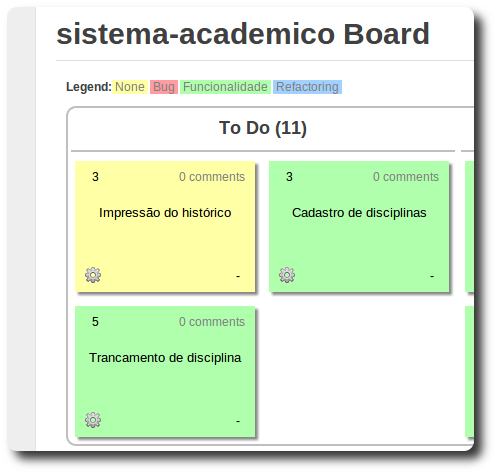
\includegraphics[scale=0.5]{images/count-points}
  \label{img:count-points}
\end{figure}

Contudo, a utilização desta técnica deve ser feita com cautela. Quando se utiliza \textit{stubs} em demasia, cria-se um acoplamento muito grande entre teste e implementação. Por exemplo, se na implementação do método \texttt{count\_points} for preciso fazer uso de mais algum atributo de \textit{Task} (em uma refatoração, por exemplo), o \textit{stub} também deverá possuir esse atributo, fazendo com que o teste tenha que ser alterado. Isso vai contra uma das premissas da refatoração de que se o comportamento do método não é modificado, seu teste deve permanecer o mesmo e continuar passando após ser feita a alteração na implementação.

É importante notar a diferença entre os \textit{stubs} e as estratégias de \textit{fixture replacement}\footnote{\textit{Fixture replacement} é uma técnica que tem como objetivo separar a inicialização do teste de sua codificação em si, dando a possibilidade de se criar objetos com estados pré-definidos que possam ser reutilizados em mais de um teste.} baseadas em instâncias. Nestas estratégias, o \textit{fixture} é um objeto real da classe. Assim, um objeto criado via \textit{fixture replacement} de instância, fica sujeito a detalhes de sua implementação da classe real. Dessa forma, o {fixture} não cria o isolamento que um \textit{stub} em seu lugar criaria, pois o stub simplesmente simula uma instância e, portanto, não fica sujeito comportamentos inesperados.


\subsection{Contextualizando o \textit{mock}}
\label{sub:contextualizando_o_mock}

De modo semelhante ao código \ref{code:todo} apresentado na Seção \ref{sub:a_ubiquidade_do_tdd}, o código \ref{code:mock} apresenta a implementação de um método de \textit{controller} que é chamado via AJAX (\textit{Asynchronous Javascript and XML})\nomenclature{AJAX}{Asynchronous Javascript and XML} e implementa a atualização dos responsáveis por uma tarefa diretamente do kanban do projeto, como apresentado na figura \ref{img:edit-contributors}. Além atualizar os responsáveis pela tarefa tarefa na base de dados, este método captura, trata e envia informações para que a interface do kanban seja atualizada. Este é outro caso onde um experimento foi para produção, sem testes e com um código ruim. Desta forma, neste caso não foi utilizado TDD para criar os testes, sendo estes escritos após a implementação.

\newpage

\begin{mycode}{ruby}%
{Código do método que atualiza os responsáveis por uma tarefa assincronamente}{code:mock}
# app/controllers/boards_controller.rb
class BoardsController < InheritedResources::Base
  # TODO: Make test and refactor
  def update_assignees
    task = Task.find(params[:task_id])
    params[:assignees].delete "-"
    params[:assignees] = nil if params[:assignees].empty?
    task.update_attribute(:contributor_ids, params[:assignees])

    if params[:assignees].nil?
      assignees_sentence = "-"
    else
      assignees_sentence = task.contributors.collect(&:username).to_sentence
    end

    if assignees_sentence.length > 25
      long_sentence = true
      assignees_long_sentence = assignees_sentence
      assignees_sentence = assignees_sentence.truncate(25)
    end

    data = { :assignees_sentence => assignees_sentence,
             :long_sentence => long_sentence,
             :assignees_long_sentence => assignees_long_sentence }
    render :text => data.to_json
  end
end
\end{mycode}

\begin{figure}[h]
  \center
  \caption{Atualização dos responsáveis pela tarefa diretamente no kanban do projeto}
  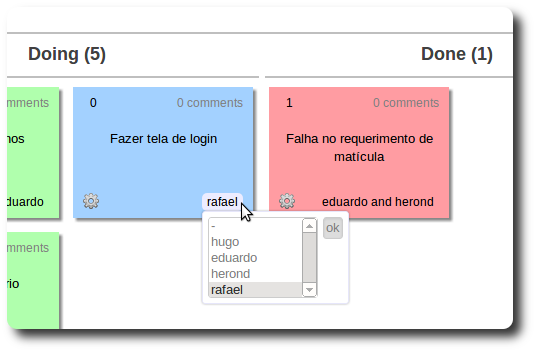
\includegraphics[scale=0.55]{images/edit-contributors}
  \label{img:edit-contributors}
\end{figure}

O teste para o método \texttt{update\_assignees}, com a utilização de \textit{mock}, é apresentado no código \ref{code:mock_spec_mockista}. Como o teste quer validar a funcionalidade para mais de um responsável (\textit{assignees}), são criados dois objetos mockados da classe \textit{Contributor}, além de também ser necessário cria um objeto mockado da classe \textit{Task}. Com esses 3 objetos mockados, está feito a \textit{setup} para o teste.

Em seguida verificadas as chamadas à métodos sobre os objetos mockados. Isto é feito através do método \texttt{should\_receive} que recebe como parâmetro o método a ser chamado. Em seguida, pode ser aninhado o método \texttt{with} que recebe os parâmetros que devem ser passados para o método chamado no \texttt{should\_receive}. Para finalizar a cadeia, pode ser ainda aninhado o método \texttt{and\_return} que indica o retorno do método chamado no \texttt{should\_receive}.

Por fim, através de um \texttt{get}, é feita a chamada ao método do \textit{controller} testado (\texttt{update\_assignees}), e é verificado se a resposta obtida está de acordo com as expectativas.

\begin{mycode}{rspec}%
{Teste utilizando \textit{mock} para o método \texttt{update\_assignees}}{code:mock_spec_mockista}
# spec/controllers/boards_controller_spec.rb
describe BoardsController do
  context "should update task assignees" do
    it "with more than one assignee" do
      task = mock_model(Task)
      hugo = mock_model(Contributor, :id => "5", :username => "hugomaiavieira")
      rodrigo = mock_model(Contributor, :id => "9", :username => "rodrigomanhaes")

      Task.should_receive(:find).with("1").and_return(task)
      task.should_receive(:update_attribute).
        with(:contributor_ids, ["5", "9"]).and_return(true)
      task.should_receive(:contributors).and_return([hugo, rodrigo])

      get :update_assignees, :task_id => "1", :assignees => ["5", "9"]

      response.body.should ==
        { :assignees_sentence => "hugomaiavieira and rod...",
          :long_sentence => true,
          :assignees_long_sentence => "hugomaiavieira and rodrigomanhaes" }.to_json
    end
  end
end
\end{mycode}

O grande problema do mock está nas verificações de chamada à métodos dos objetos mockados. Pose-se perceber que está se verificando a ordem em que os métodos são chamados, bem como os parâmetros passados. Desta forma, na realidade, está se testando \textbf{como} a funcionalidade está sendo implementada e não \textbf{o que} ela faz \cite{UnitForAReason}. Com isso, o acoplamento entre o teste e a implementação torna-se extremamente grande, ainda maior do que com a utilização de \textit{stubs}. Qualquer refatoração mínima feita na implementação, mesmo que não interfira em seu comportamento, pode fazer com que os testes quebrem.

Um exemplo para este problema seria trocar o método \texttt{find} na linha 5 do código \ref{code:mock} pelo método \texttt{find\_by\_id}. Com essa troca, o comportamento do método \texttt{update\_assignees} continua o mesmo, porém, o teste quebraria na linha 9 do código \ref{code:mock_spec_mockista} informado que a classe \texttt{Task} esperava receber o método \texttt{find} mas recebeu o método \texttt{find\_by\_id}.

Para fazer uma comparação, no código \ref{code:mock_spec_tradicional} é apresentado um outro teste para o mesmo exemplo, porém, utilizando objetos reais criados através de \textit{fixture replacement}. Note que desta vez foi preciso criar um objeto \textit{project} para ligar ao objeto \textit{task}, pois quando são utilizados objetos reais, todas as validações são executadas e, neste caso, uma tarefa obrigatoriamente deve estar ligada a um projeto.

\begin{mycode}{rspec}%
{Teste utilizando \textit{fixture replacement} para o método \texttt{update\_assignees}}{code:mock_spec_tradicional}
# spec/controllers/boards_controller_spec.rb
describe BoardsController do
  context "should update task assignees" do
    it "with more than one assignee" do
      project = Factory.create :project
      task = Factory.create :task, :project => project
      hugo = Factory.create :contributor, :username => "hugomaiavieira"
      rodrigo = Factory.create :contributor, :username => "rodrigomanhaes"

      get :update_assignees, :task_id => task.id, :assignees => [hugo.id, rodrigo.id]

      response.body.should ==
        { :assignees_sentence => "hugomaiavieira and rod...",
          :long_sentence => true,
          :assignees_long_sentence => "hugomaiavieira and rodrigomanhaes" }.to_json
    end
  end
end
\end{mycode}

Percebe-se que o teste sem o uso do \textit{mock} fica mais simples e menos acoplado à implementação. Contudo, o teste usando \textit{mock} ganhou um isolamento maior por não ficar sujeito a detalhes da implementação das classes, irrelevantes para o teste. Além disso, os testes utilizando mock rodaram com uma velocidade 58\% maior do que o teste sem \textit{mock}. Isso acontece porque os testes sem \textit{mock} (utilizando \textit{fixture replacement}) fazem acesso ao disco para gravar as informações dos objetos reais no banco de dados de teste.


\subsection{A dicotomia entre o TDD clássico e o mockista}
\label{sub:tdd_classico_e_mockista}

\citeonline{MocksArentStubs} generaliza os dublês de teste como \textit{mocks} e define duas faces da sua utilização com TDD, onde o divisor é \textbf{quando} utilizar um dublê:

\begin{itemize}
  \item O estilo \textbf{TDD clássico} é o qual se utiliza objetos reais sempre que possível e dublês quando é complicado utilizar o real.

  \item O estilo \textbf{TDD mockista} (\textit{mockist}, em inglês) é o qual se utiliza dublês sempre.
\end{itemize}

Como visto anteriormente, a utilização de dublês de teste, em alguns casos, é claramente benéfica para o projeto. Porém, seu uso excessivo pode causar um problema de acoplamento entre o teste e a implementação.

\citeonline{ArtOfAgileDevelopment} afirma o \textit{mock} é uma técnica útil, e as vezes é a melhor maneira de testar o código. No entanto, ele diz que antes de assumir que o \textit{mock} é apropriado para a situação, deve-se olhar novamente para o design do código, pois pode ser uma oportunidade de aprimoramento.

Uma outra questão a ser levada em consideração é que quando não se utiliza dublês, está se testando a integração entre as classes, e isso pode ter um efeito colateral positivo, capturando erros que muitas vezes passam despercebidos ao se utilizar \textit{dublês}. Contudo, quando não se utiliza dublês, para testar uma unidade pode ser necessário desenvolver outras unidades colaboradoras, cada qual com seus correspondentes testes de unidade, assim tirando o foco da tarefa corrente.

Dessa forma, assim como \citeonline{MocksArentStubs} conclui, não existe razão para adotar um estilo TDD mockista, sendo o TDD clássico a melhor opção, utilizando os dublês de teste de forma controlada.
  \chapter{Conclusões} % (fold)
\label{cha:conclusoes}

\textbf{TODO: refazer todo esse capítulo}

O presente trabalho discutiu e contextualizou as mais importantes técnicas de emergentes de teste de software, sendo elas TDD, BDD, Integração Contínua e Dublês de Teste, fazendo uma ``revisão crítica"\ das mesmas e construindo conhecimento em cima de informações ainda dispersas e não sistematizadas.

Discutiram-se aqui, além de uma revisão bibliográfica de agilismo, temas de pouca ou nenhuma sistematização acadêmica, como legibilidade de testes automatizados, comparação entre modelos de escrita de testes de aceitação, a pertinência da utilização de técnicas de \textit{test-first programming} como TDD em diferentes contextos, problemas no uso de dublês de teste, entre outros. Além disto, a discussão foi contextualizada com exemplos originados de uma aplicação real, o projeto kanban-roots.

Por serem técnicas e conceitos que emergiram no meio empresarial, tendo recentemente uma maior aceitação e difusão, ainda não existe muita reflexão acadêmica sobre as mesmas. Desta forma, este trabalho contribuiu com a introdução de tais ideias na academia, abordando as mesmas de forma contextualizada.

% chapter conclusoes (end)

  \anexo
  \chapter{A efetividade do TDD}
\label{cha:a_efetividade_do_tdd}

Existem dúvidas sobre a real efetividade do TDD no que diz respeito à qualidade do código, redução de defeitos e ao aumento ou diminuição da produtividade. Empiricamente, é comum observar a sensação subjetiva, contudo, por ser um processo complexo, é muito difícil avaliar e chegar a uma conclusão exata sobre os ganhos e benefícios de toda e qualquer prática em engenharia de software.

Nos últimos anos, vem sendo feitos alguns experimentos para tentar mostrar de maneira empírica que TDD realmente é efetivo no processo de desenvolvimento de software.

\section{Estudos na indústria}
\label{sec:estudos_na_industria}

Um estudo feito por \citeonline{MaximilienTDD}, fazendo um comparativo de entre o desenvolvimento pré e pós a utilização do TDD, mostrou uma redução de 50\% na taxa de defeitos encontrados no sistema, tendo um mínimo impacto negativo na produtividade da equipe. Além disso, foi percebido que a utilização do TDD os fez produzir um produto que incorporaria mais facilmente alterações posteriores.

Outro estudo feito por \citeonline{ChinaTDD} dividiu dois grupos, um utilizando TDD e outro utilizando Test-last\footnote{Nesta abordagem os testes escritos após o código.}. O estudo mostrou que o time que utilizou TDD produziu menos defeitos e quando estes ocorriam, eram capazes de solucioná-los muito mais rapidamente. No estudo realizado por \citeonline{DammTDD} também é mostrada uma redução nas taxas de defeito.

Já o estudo feito por \citeonline{GeorgeTDD} mostrou que, apesar de TDD poder reduzir inicialmente a produtividade dos desenvolvedores em 16\%, o código produzido apresentou uma cobertura entre 92\% a 98\%. Além disso, uma análise qualitativa mostrou que 87.5\% dos programadores acreditam que TDD facilitou o entendimento dos requisitos e 95.8\% acreditam que TDD reduziu o tempo gasto com \textit{debug}. 78\% também acreditam que TDD aumentou a produtividade da equipe. No entanto, apenas metade dos desenvolvedores acreditam que TDD leva a uma diminuição do tempo de desenvolvimento. Sobre qualidade, 92\% acreditam que TDD ajuda a manter um código de maior qualidade e 79\% acreditam que ele promove um design mais simples e 71\% acreditam que esta abordagem é notavelmente efetiva. Portanto, agregando todos esses dados, o estudo mostra que 80\% dos desenvolvedores acreditam que o uso do TDD é realmente efetivo.

\citeonline{EmpiricalTDD} realizaram um estudo de caso conduzidos em três times na Microsoft e um na IBM. Os resultados indicaram que o número de defeitos diminuiu entre 40\% e 90\% em relação à projetos similares que não usaram TDD. Contudo, o estudo mostrou também que a utilização do TDD aumentou o tempo inicial de desenvolvimento entre 15\% e 35\%.


\section{Estudos na academia}
\label{sec:estudos_na_academia}

Um estudo feito por \citeonline{JanzenTDD} dividiu um conjunto de alunos em três grupos, onde cada um deles utilizaria uma abordagem distinta. Um grupo utilizou TDD, o outro Test-last e o último não fazia testes. O grupo que utilizou TDD produziu e por volta de duas vezes  mais funcionalidades que os outros dois grupos e com um número similar de defeitos. Além disso, o grupo que utilizou TDD foi o único a completar a interface gráfica. Apesar de ter desenvolvido mais funcionalidades, o grupo que utilizou TDD investiu a mesma quantidade de tempo dos demais grupos para o desenvolvimento.

O Grupo TDD despendeu menos esforço por linha de código e despendeu 88\% menos esforço por funcionalidade do que o grupo que não fez testes, e 57\% menos esforço por funcionalidade do que o grupo Test-last. Além disso, o grupo TDD teve uma cobertura de testes 86\% maior do que o grupo Test-last.

Também foi feita uma micro-avaliação somente do grupo TDD, sendo aferido que nas partes do código para os quais foram feitos testes, a complexidade foi 43\% menor do que as partes sem testes. Além disso, as classes testadas tiveram um acoplamento 104\% menor do que as não testadas.

Já o estudo feito por \citeonline{ErdogmusTDD} com vinte e quatro alunos de graduação mostrou que a utilização do TDD fez com que houvesse um aumento na produtividade, além de reduzir a necessidade de \textit{debug} e retrabalho. Entretanto nenhuma diferença na qualidade no código foi encontrada.


\section{Conclusões a partir dos estudos}
\label{sec:conclusoes_efetividade_tdd}

A maioria dos experimentos feitos tanto na indústria quanto na academia mostra que TDD melhora o processo de desenvolvimento de software, aumentando a qualidade do código, reduzindo o número de defeitos e diminuindo o tempo gasto com depuração.

Contudo existe uma divergência em relação à produtividade dos desenvolvedores. Os estudos na indústria mostram que o uso do TDD faz com que a produtividade diminua um pouco, diferente dos estudos na academia que mostram um aumento na produtividade. Uma possível conclusão sobre a causa desta divergência é que os desenvolvedores na indústria já utilizam há algum tempo um outro modelo de desenvolvimento e estão acostumados com ele, fazendo com que a mudança para o TDD inicialmente seja um pouco complicada. Isso já não é verdade quando se está falando de alunos de graduação, que não têm que realizar uma mudança de paradigma como os profissionais na indústria neste caso.

Uma outra questão sobre a diminuição da produtividade apresentada nos estudos da indústria, é que essa produtividade tem uma queda maior no início, quando os desenvolvedores ainda estão se acostumando com a técnica e as mudanças no código são constantes. Contudo, com o passar do tempo e o amadurecimento do projeto, essa produtividade tende a ser maior do que sem a utilização do TDD, pois os desenvolvedores já aprenderam e acostumaram com a técnica e, com uma cobertura de testes maior e com código de melhor qualidade, modificações no código são mais simples e rápidas de serem feitas.

Durante o desenvolvimento do kanban-roots não foi realizado nenhum experimento semelhante aos apresentados nos tópicos anteriores. Uma vez que este trabalho se direciona à exposição e à discussão de técnicas emergentes de desenvolvimento de software, aplicadas à construção de software real, tais experimentos, trazidos aqui a título de informação e enriquecimento, fugiriam ao escopo do presente trabalho. Cabe ressaltar, entretanto, que a melhoria na qualidade do código e na diminuição de defeitos, citada pelos estudos, foi percebida subjetivamente pelo autor no decorrer do processo de desenvolvimento do software. Além disto, conforme citado na Seção \ref{sub:a_ubiquidade_do_tdd}, apenas dois defeitos foram encontrados no kanban-roots em produção, ambos em trechos de código não cobertos por testes. Ou seja, onde a aplicação de TDD não foi realizada de modo estrito.
  \chapter{Códigos do comparativo entre texto plano e código puro}
\label{cha:codigo_do_comparativo}

\begin{mycode}{cucumber}%
{Conjunto de especificações em texto plano}{code:bdd_cucumber_comparativo}
Feature: Run a group of scenarios
  As a user
  I want to run a group of scenarios
  In order to compare with pure code specs

  Scenario: Comments should be rendered with Markdown syntax on the tasks page
    Given I am a contributor of "sgtran" project
    And I am authenticated
    And I have a task of "sgtran" project
    When I am on the task page
    And I fill in "comment_content" with "# Some content [link](http://exemplo.com)"
    And I press "Comment"
    Then I should see "Some content" in a "h1" tag
    And I should see "link" in an "a" tag

  Scenario: Sign out
    Given I am an authenticated contributor
    And I am on the dashboard
    When I follow "Sign out"
    Then I should see "Sign in"

  Scenario: Register new project
    Given I am an authenticated contributor
    And I am on the new project page
    When I fill in "Name" with "name-1"
    And I fill in "Description" with "description 1"
    And I press "Save"
    Then I should be the project's owner
    And I should be on the projects board page
    And I should see "name-1 Board"

  Scenario: Try to register projects with erros
    Given I am an authenticated contributor
    And I am on the new project page
    And I press "Save"
    Then I should see "can't be blank"
    And I should not have any project

  Scenario: Edit a project
    Given I am an authenticated contributor
    And I have a project
    When I am on the project edit page
    And I fill in "Name" with "Some_name"
    And I fill in "Description" with "Any description"
    And I press "Save"
    Then I should be on the projects board page
    And I should see "some_name Board"

  Scenario: Delete project
    Given I am an authenticated contributor
    And the following projects:
      | name   | description   |
      | name_1 | description 1 |
      | name_2 | description 2 |
      | name_3 | description 3 |
      | name_4 | description 4 |
    When I delete the 3rd project
    And I am on the dashboard page
    Then I should see "name_1"
    And I should see "name_2"
    And I should see "name_4"
    And I should not see "name_3"

  Scenario: Register a category successfully
    Given I am a contributor of "sgtran" project
    And I am authenticated
    And I am on the "sgtran" categories page
    When I follow "New Category"
    And I fill in "Name" with "Feature"
    And I fill in "Color" with "ffa5a5"
    And I press "Save"
    Then I should see "Category was successfully created."
    And I should see "Feature"
    And I should see "ffa5a5"
    And "sgtran" project should have "1" category

  Scenario Outline: Try to register categories with errors
    Given I am a contributor of "sgtran" project
    And I am authenticated
    And I am on the "sgtran" categories page
    And I have a category with name "Bug" and color "ffa5a5"
    When I follow "New Category"
    And I fill in "Name" with "<name>"
    And I fill in "Color" with "<color>"
    And I press "Save"
    Then I should see "<sentence>"
    And "sgtran" project should have "1" category

    Examples:
    | name    | color  | sentence                   |
    |         | a5d2ff | can't be blank             |
    | Feature |        | can't be blank             |
    | Feature | ffa5a5 | should be uniq for project |
    | Bug     | a5d2ff | should be uniq for project |
    | Bug     | red    | is invalid                 |
    | Bug 1   | a5d2ff | is invalid                 |

  Scenario: Edit a category
    Given I am a contributor of "sgtran" project
    And I am authenticated
    And I have a category with name "Feature" and color "ffa5a5"
    When I am on the category edit page
    And I fill in "Name" with "New feature"
    And I press "Save"
    Then I should see "New feature"
    And I should see "Category was successfully updated."

  Scenario: Register contributors successfully
    Given I am on the new contributor page
    When I fill in "Name" with "Someone of Nothing"
    And I fill in "Username" with "someone"
    And I fill in "E-mail" with "someone@gmail.com"
    And I fill in "Password" with "password"
    And I fill in "Password confirmation" with "password"
    And I press "Sign up"
    Then I should see "You have signed up successfully."

  Scenario Outline: Try to register contributors with errors
    Given I am on the new contributor page
    When I fill in "Name" with "<name>"
    And I fill in "Username" with "<username>"
    And I fill in "E-mail" with "<e-mail>"
    And I fill in "Password" with "password"
    And I fill in "Password confirmation" with "password"
    And I press "Sign up"
    Then I should see "<sentence>"

    Examples:
    | name    | username | e-mail            | sentence       |
    |         | someone  | someone@gmail.com | can't be blank |
    | Someone |          | someone@gmail.com | can't be blank |
    | Someone | someone  |                   | can't be blank |
    | Someone | someone  | someone@nothing   | is invalid     |

  Scenario: Edit a contributor
    Given I am contributor with password "123456" and email "test@test.com"
    And I am authenticated
    And I am on my details edit page
    And I fill in "Username" with "hugomaiavieira"
    And I fill in "Current password" with "123456"
    And I press "Save"
    Then I should see "hugomaiavieira"

  Scenario: Sign in with username successfully
    Given I am contributor with password "123456" and username "someone"
    Given I am on the sign in page
    When I fill in "Login" with "someone"
    And I fill in "Password" with "123456"
    And I press "Sign in"
    Then I should see "Signed in successfully."

  Scenario: Sign in with email successfully
    Given I am contributor with password "123456" and email "someone@example.com"
    Given I am on the sign in page
    When I fill in "Login" with "someone@example.com"
    And I fill in "Password" with "123456"
    And I press "Sign in"
    Then I should see "Signed in successfully."
\end{mycode}

\begin{mycode}{rspec}%
{Conjunto de especificações em código puro}{code:bdd_rspec_comparativo}
require 'spec_helper'

feature 'Authentication' do
  it 'sign out' do
    contributor = Factory.create :contributor
    login(contributor.email, contributor.password)
    click_link 'Sign out'
    page.should have_content 'Sign in'
  end
end

feature 'validates uniqueness of name for contributor' do
  background do
    @hugo = Factory.create :contributor
    @project = Factory.create :project, :name => 'kanban-roots', :owner => @hugo
  end

  scenario 'when edit' do
    login(@hugo.email, @hugo.password)
    visit edit_project_path(@project)
    click_button 'Save'
    page.should have_content 'Project was successfully updated.'
  end

  scenario 'when create' do
    login(@hugo.email, @hugo.password)
    visit new_project_path
    fill_in 'Name', :with => 'kanban-roots'
    click_button 'Save'
    page.should have_content 'you already have a project with this name'
    click_link 'Sign out'

    dudu = Factory.create :contributor
    login(dudu.email, dudu.password)
    visit new_project_path
    fill_in 'Name', :with => 'kanban-roots'
    click_button 'Save'
    page.should have_content 'Project was successfully created.'
  end
end

feature 'manipulate projects' do
  context 'register a new project' do
    before do
      @contributor = Factory.create :contributor
      login @contributor.email, @contributor.password
    end

    it 'successfully' do
      visit new_project_path
      fill_in 'Name', :with => 'name-1'
      fill_in 'Description', :with => 'description 1'
      click_button 'Save'
      page.should have_content 'Project was successfully created.'
      project = Project.all.last
      project.owner.should == @contributor
      current_path.should == project_board_path(project)
      within('h1') do
        page.should have_content 'name-1 Board'
      end
    end

    it 'with errors' do
      visit new_project_path
      click_button 'Save'
      within('form > div[2]') do
        page.should have_content "can't be blank"
      end
      @contributor.projects.should be_empty
    end
  end

  it 'edit a project successfully' do
    contributor = Factory.create :contributor
    project = Factory.create :project, :owner => contributor
    login contributor.email, contributor.password
    visit edit_project_path(project)
    fill_in 'Name', :with => 'Some_name'
    fill_in 'Description', :with => 'Some description'
    click_button 'Save'
    page.should have_content 'Project was successfully updated.'
    current_path.should == project_board_path(project)
    within('h1') do
      page.should have_content 'some_name Board'
    end
  end

  it 'delete a project' do
    contributor = Factory.create :contributor
    projects = []
    5.times do |i|
      projects << (Factory.create :project, :owner => contributor,
                                :name => "name_#{i}", :description => "description #{i}")
    end
    login contributor.email, contributor.password

    visit project_board_path(projects[2])
    click_link 'Admin'
    click_link 'Destroy'
    page.should have_content projects[0].name
    page.should have_content projects[1].name
    page.should_not have_content projects[2].name
    page.should have_content projects[3].name
    page.should have_content projects[4].name
  end
end

feature 'Manage categories' do
  before do
    @project = Factory.create :project
    @contributor = Factory.create :contributor, :contributions => [@project]
    @project.update_attribute(:contributors, [@contributor])
    login @contributor.email, @contributor.password
  end

  context 'register a category' do
    it 'successfully' do
      visit project_categories_path(@project)
      click_link 'New Category'
      fill_in 'Name', :with => 'Feature'
      fill_in 'Color', :with => 'ffa5a5'
      click_button 'Save'
      page.should have_content 'Category was successfully created.'
      page.should have_content 'Feature'
      page.should have_content 'ffa5a5'
      @project.reload.categories.length.should == 1
    end

    context 'with error' do
      before do
        visit project_categories_path(@project)
        click_link 'New Category'
      end

      it 'blank fields' do
        fill_in 'Color', :with => ''
        click_button 'Save'
        within('form > div[2]') { page.should have_content "can't be blank" }
        within('form > div[3]') { page.should have_content "can't be blank" }
      end

      context 'uniq for project' do
        before do
          @category = Factory.create :category, :project => @project,
                                       :color => 'ffa5a5', :name => 'Bug'
        end

        it 'name' do
          fill_in 'Name', :with => 'Bug'
          fill_in 'Color', :with => 'a5d2ff'
          click_button 'Save'
          within('form > div[2]') { page.should have_content 'should be uniq for project' }
        end

        it 'color' do
          fill_in 'Name', :with => 'Feature'
          fill_in 'Color', :with => 'ffa5a5'
          click_button 'Save'
          within('form > div[3]') { page.should have_content 'should be uniq for project' }
        end
      end

      context 'invalid' do
        it 'name' do
          fill_in 'Name', :with => 'Bug 1'
          fill_in 'Color', :with => 'a5d2ff'
          click_button 'Save'
          within('form > div[2]') { page.should have_content 'is invalid' }
        end

        it 'color' do
          fill_in 'Name', :with => 'Bug'
          fill_in 'Color', :with => 'red'
          click_button 'Save'
          within('form > div[3]') { page.should have_content 'is invalid' }
        end
      end
    end
  end

  it 'edit a category' do
    category = Factory.create :category, :project => @project,
                                :name => 'Feature', :color => 'ffa5a5'
    visit edit_project_category_path(@project, category)
    fill_in 'Name', :with => 'New feature'
    click_button 'Save'
    page.should have_content 'New feature'
    page.should have_content 'Category was successfully updated.'
  end
end

feature 'Manipulate contributors' do
  context 'register a contributor' do
    it 'successfully' do
      visit new_contributor_registration_path
      fill_in 'Name', :with => 'Someone of Nothing'
      fill_in 'Username', :with => 'someone'
      fill_in 'E-mail', :with => 'someone@gmail.com'
      fill_in 'Password', :with => 'password'
      fill_in 'Password confirmation', :with => 'password'
      click_button 'Sign up'
      page.should have_content 'You have signed up successfully.'
    end

    context 'with errors' do
      it 'blank fields' do
        visit new_contributor_registration_path
        click_button 'Sign up'
        within('form > div[2]') { page.should have_content "can't be blank"}
        within('form > div[3]') { page.should have_content "can't be blank"}
        within('form > div[4]') { page.should have_content "can't be blank"}
        within('form > div[5]') { page.should have_content "can't be blank"}
      end

      it 'invalid' do
        visit new_contributor_registration_path
        fill_in 'E-mail', :with => 'someone@nothing'
        click_button 'Sign up'
        within('form > div[4]') { page.should have_content "is invalid"}
      end
    end
  end

  context 'edit a contributor' do
    before do
      @contributor = Factory.create :contributor
      login @contributor.email, @contributor.password
    end

    it 'successfully' do
      visit edit_contributor_registration_path
      fill_in 'Username', :with => 'hugomaiavieira'
      fill_in 'Current password', :with => '123456'
      click_button 'Save'
      page.should have_content 'hugomaiavieira'
    end

    it 'current password invalid' do
      visit edit_contributor_registration_path
      fill_in 'Username', :with => 'hugomaiavieira'
      fill_in 'Current password', :with => '123456789'
      click_button 'Save'
      within('form > div[7]') { page.should have_content 'is invalid' }
    end
  end
end

feature 'Sign in successfully' do
  it 'with username' do
    contributor = Factory.create :contributor, :username => 'someone'
    login contributor.username, contributor.password
    page.should have_content 'Signed in successfully.'
  end

  it 'with e-mail' do
    contributor = Factory.create :contributor, :email => 'someone@example.com'
    login contributor.email, contributor.password
    page.should have_content 'Signed in successfully.'
  end
end
\end{mycode}

  %--------------------------------- Bibliografia ------------------------------

  \citeoption{abnt-repeated-author-omit=yes}
  \bibliographystyle{abnt-alf}
  \bibliography{bibliografia}
\end{document}